\documentclass[12pt]{report}
\usepackage[utf8]{inputenc}
\usepackage[T1]{fontenc}
\usepackage{hyperref}
\usepackage{graphicx}
\usepackage{listings}
\usepackage{xcolor}
% Define JSON language for listings
\lstdefinelanguage{json}{
    basicstyle=\ttfamily\small,
    numbers=left,
    numberstyle=\tiny,
    stepnumber=1,
    numbersep=5pt,
    showstringspaces=false,
    breaklines=true,
    frame=lines,
    backgroundcolor=\color{gray!10},
    literate=
     *{0}{{{\color{blue}0}}}{1}
      {1}{{{\color{blue}1}}}{1}
      {2}{{{\color{blue}2}}}{1}
      {3}{{{\color{blue}3}}}{1}
      {4}{{{\color{blue}4}}}{1}
      {5}{{{\color{blue}5}}}{1}
      {6}{{{\color{blue}6}}}{1}
      {7}{{{\color{blue}7}}}{1}
      {8}{{{\color{blue}8}}}{1}
      {9}{{{\color{blue}9}}}{1}
      {:}{{{\color{red}:}}}{1}
      {,}{{{\color{red},}}}{1}
      {"}{{{\color{orange}"}}}{1},
}
\usepackage{amsmath}
\usepackage{geometry}
\usepackage{parskip}
\usepackage{fancyhdr}
\usepackage{lastpage}
\usepackage{textcomp} % For \textrupee{}
\usepackage{booktabs} % For \toprule, \midrule, \bottomrule
\usepackage{amssymb}  % For \approx symbol
\usepackage{float}
\usepackage{draftwatermark}
\geometry{margin=1in}

% Configure CONFIDENTIAL watermark
\SetWatermarkText{CONFIDENTIAL}
\SetWatermarkScale{1.5}
\SetWatermarkColor[gray]{0.8}
\SetWatermarkAngle{45}

% Define rupee symbol if not available
\newcommand{\rupee}{\textrupee{}}

% Configure fancy headers and footers
\pagestyle{fancy}
\fancyhf{} % Clear all header and footer fields

% Add logo to header on every page
\fancyhead[L]{
\includegraphics[height=0.8cm]{../../pics/logo.png}}
\fancyhead[R]{\textbf{AI Agent Module - Software Design Document v1.0}}
\fancyfoot[L]{Dhvani Analytic Intelligence Pvt. Ltd.}
\fancyfoot[C]{\thepage\ of \pageref{LastPage}}
\fancyfoot[R]{\today}

% Adjust header rule
\renewcommand{\headrulewidth}{0.4pt}
\renewcommand{\footrulewidth}{0.4pt}

% Custom title page
\title{
  \vspace{-2cm}
  \begin{center}
    
\includegraphics[width=6cm]{../../pics/logo.png}\\[2cm]
    {\Huge \textbf{Software Design Document}}\\[0.5cm]
    {\Large AI Agent Module}\\[1cm]
    {\large For Prowiz ERP System}\\[1.5cm]
    {\normalsize \textbf{Version 1.0}}\\[0.5cm]
    {\small Document ID: SDD-AI-001}
  \end{center}
}
\author{
  \textbf{Nithin Vadekkapat}\\
  Director-AI\\[0.5cm]
  \textbf{Dhvani Analytic Intelligence Pvt. Ltd.}\\
  AI Solutions Division
}
\date{\today}

\begin{document}

% Title page with no header/footer
\thispagestyle{empty}
\maketitle
\newpage

% Document revision history
\thispagestyle{empty}
\section*{Document Revision History}
\begin{table}[h]
\centering
\begin{tabular}{|c|c|c|l|}
\hline
\textbf{Version} & \textbf{Date} & \textbf{Author} & \textbf{Description} \\
\hline
1.0 & July 3, 2025 & Nithin Vadekkapat & Initial version \\
\hline
\end{tabular}
\end{table}
\vfill
\newpage

% Table of contents with no header/footer
\thispagestyle{empty}
\tableofcontents
\clearpage

% Start fancy page style for content pages
\pagestyle{fancy}

\chapter{Introduction}
\section{Purpose}
The purpose of the AI Agent Module is to provide a set of specialized agents that can autonomously perform tasks related to process design and documentation. The module aims to streamline workflows, improve accuracy, and enhance collaboration across teams. Key functionalities include:
\begin{itemize}
  \item \textbf{Preprocesses the image}: Enhances image quality, adjusts contrast, and optimizes resolution for analysis
  \item \textbf{Detects symbols and equipment}: Uses computer vision to identify pumps, valves, vessels, and instrumentation
  \item \textbf{Extracts text labels}: Applies OCR to extract equipment tags, specifications, and process parameters
  \item \textbf{Maps spatial relationships}: Analyzes the positioning and connections between identified components
  \item \textbf{Builds process graph}: Constructs a NetworkX graph representing the complete process topology
  \item \textbf{Generates structured outputs}: document presents the detailed software design for the AI Agent Module within the Prowiz ERP system. It describes the architecture, interfaces, and operational workflows for each specialized agent.
\end{itemize}
\section{Scope}
The scope of this document covers:
\begin{itemize}
  \item Functional responsibilities of each AI agent (Compliance, Document Generation, Diagram Parsing, Email, ERP-Chat).
  \item Scope and boundaries for each agent (what each agent handles vs. out of scope).
  \item Example use cases demonstrating invocation and outputs for each agent.
\end{itemize}

\chapter{Overall Architecture}
\section{Module Overview}
The AI Agent Module exposes a REST/GRPC API, orchestrates incoming requests via a central orchestrator, and dispatches tasks to individual agent services. It leverages a shared LLM runtime, embedding service with Vector DB, a project-scoped Knowledge Base, a message queue for resilience, and observability via Prometheus and Loki.

\section{System Flow Architecture}
The following diagram illustrates the complete system flow and architecture of the AI Agent Module:

\begin{figure}[htbp]
\centering
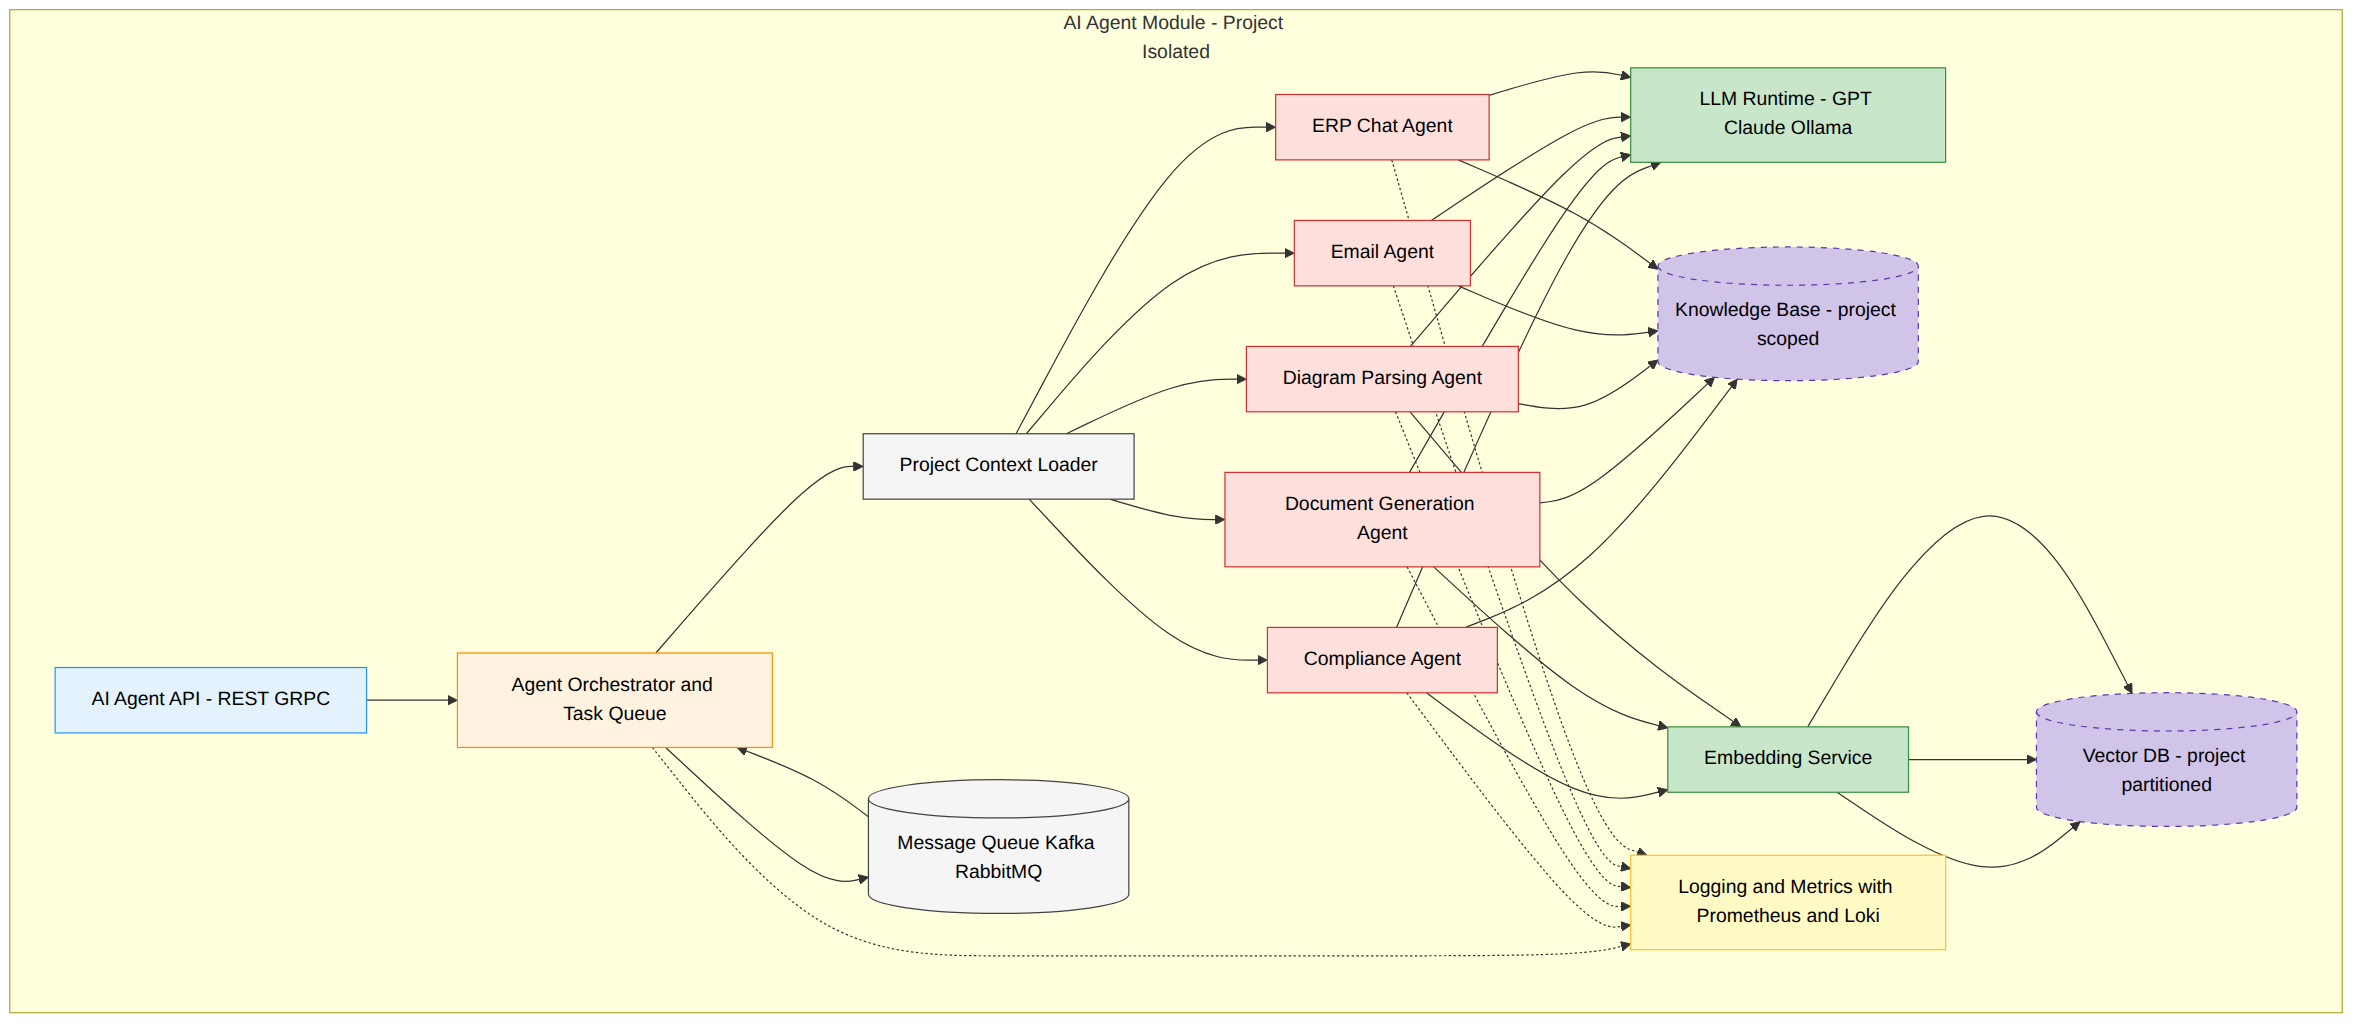
\includegraphics[width=\textwidth,height=1.2\textheight,keepaspectratio]{../../pics/flow.png}
\caption{AI Agent Module System Flow Architecture}
\label{fig:system-flow}
\end{figure}

\subsection{System Components Overview}
The AI Agent Module consists of the following key components and their functionalities:

\subsubsection{API Gateway \& Orchestrator}
\begin{itemize}
  \item Exposes REST/GRPC API endpoints for external system integration
  \item Routes incoming requests to appropriate specialized agents
  \item Manages request orchestration and workflow coordination
\end{itemize}

\subsubsection{Specialized AI Agents}
\begin{itemize}
  \item \textbf{Compliance Agent}: Validates parameters against specifications and business rules
  \item \textbf{Document Generation Agent}: Creates templated documents with data merging and narratives
  \item \textbf{Diagram Parsing Agent}: Extracts structured data from P\&ID and CAD diagrams
  \item \textbf{Email Agent}: Parses inbound emails for project instructions and attachments
  \item \textbf{ERP-Chat Agent}: Converts natural-language commands to ERP API calls
\end{itemize}

\subsubsection{Shared Infrastructure Services}
\begin{itemize}
  \item \textbf{LLM Runtime}: GPU-hosted language model processing on Kubernetes
  \item \textbf{Embedding Service \& Vector DB}: Semantic search using Faiss/Qdrant with project partitioning
  \item \textbf{Knowledge Base}: MongoDB collections with project-scoped data storage
  \item \textbf{Message Queue}: Kafka-based request handling and retry mechanisms
  \item \textbf{Observability}: Prometheus metrics and Loki logging for system monitoring
\end{itemize}

\chapter{Compliance Agent}
\section{Function}
The Compliance Agent operates within the AI Layer of the system architecture and performs AI-powered validation of structured data received from upstream preprocessing layers. It conducts knowledge-based compliance checking and rule-based validation to produce detailed compliance reports.

\begin{figure}[htbp]
\centering
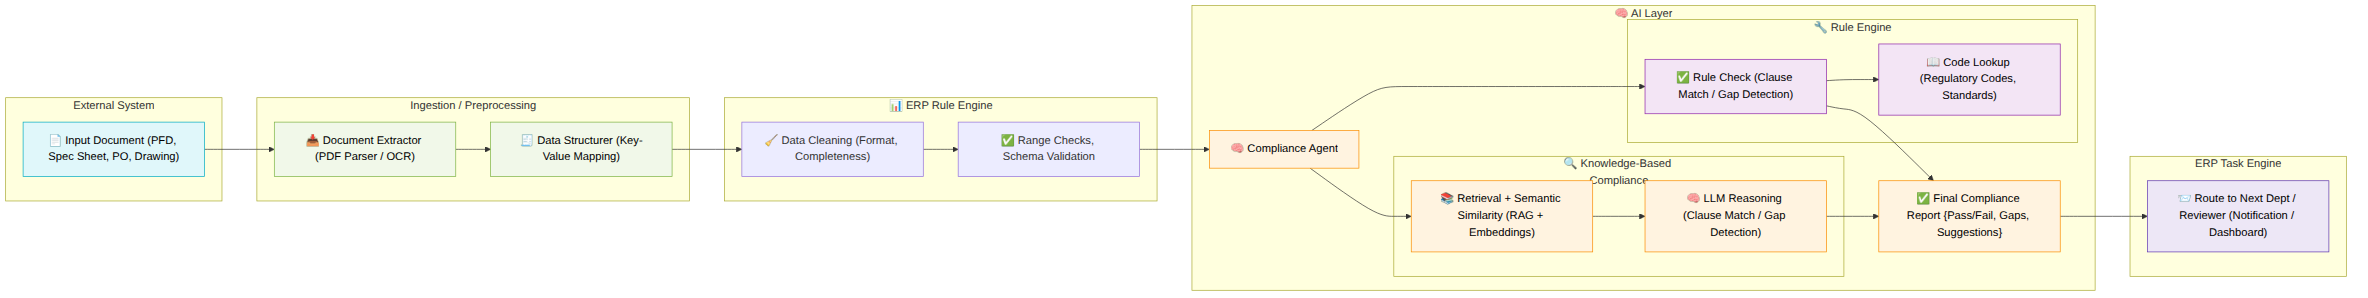
\includegraphics[width=\textwidth,height=1.2\textheight,keepaspectratio]{../../pics/compliance.png}
\caption{Compliance Agent Workflow and Architecture}
\label{fig:compliance-workflow}
\end{figure}

\section{Scope and Boundaries}
\subsection{AI Layer Scope (In-Scope)}
The Compliance Agent is responsible only for components within the \textbf{AI Layer} subgraph:
\begin{itemize}
  \item \textbf{Compliance Agent Core}: Central orchestration of AI-powered compliance validation
  \item \textbf{Knowledge-Based Compliance}: 
    \begin{itemize}
      \item RAG (Retrieval + Semantic Similarity) with embeddings
      \item LLM Reasoning for clause matching and gap detection
    \end{itemize}
  \item \textbf{Rule Engine Integration}:
    \begin{itemize}
      \item Rule-based compliance checks and clause matching
      \item Code lookup against regulatory codes and standards databases
    \end{itemize}
  \item \textbf{Structured Output Generation}: Final compliance report generation with pass/fail status, gaps, and suggestions
\end{itemize}

\subsection{External Dependencies (Out-of-Scope)}
The following components are \textbf{outside} the AI Layer and handled by other subsystems:
\begin{itemize}
  \item \textbf{External System}: Input document handling (PFDs, spec sheets, purchase orders, drawings)
  \item \textbf{Ingestion/Preprocessing Layer}: 
    \begin{itemize}
      \item Document extraction (PDF parser/OCR)
      \item Data structuring (key-value mapping)
    \end{itemize}
  \item \textbf{ERP Rule Engine Layer}:
    \begin{itemize}
      \item Data cleaning (format, completeness)
      \item Data validation (range checks, schema validation)
    \end{itemize}
  \item \textbf{ERP Task Engine}: Routing to next department/reviewer and notification systems
\end{itemize}

\subsection{Integration Boundaries}
\begin{itemize}
  \item \textbf{Input}: Receives structured, validated data from the ERP Rule Engine layer
  \item \textbf{Output}: Delivers compliance reports to the ERP Task Engine for routing
  \item \textbf{Dependencies}: Accesses shared knowledge bases and regulatory code databases
  \item \textbf{Limitations}: Cannot modify upstream data processing or downstream workflow routing
\end{itemize}

\section{Architecture Components}
The Compliance Agent operates exclusively within the AI Layer and consists of the following components:

\subsection{AI Layer Components (Compliance Agent Scope)}
\begin{itemize}
  \item \textbf{Compliance Agent Core}: Central coordinator that receives structured data from upstream layers and orchestrates AI-powered validation processes
  \item \textbf{Knowledge-Based Compliance Module}:
    \begin{itemize}
      \item \textbf{RAG System}: Retrieval and semantic similarity matching using embeddings
      \item \textbf{LLM Reasoning Engine}: Advanced reasoning for clause matching and gap detection
    \end{itemize}
  \item \textbf{Rule Engine Interface}:
    \begin{itemize}
      \item \textbf{Rule Check Processor}: Executes deterministic compliance checks
      \item \textbf{Code Lookup Service}: Interfaces with regulatory codes and standards databases
    \end{itemize}
  \item \textbf{Report Generator}: Produces structured compliance reports with pass/fail status, identified gaps, and improvement suggestions
\end{itemize}

\subsection{External Layer Dependencies (Outside AI Agent Scope)}
These components are managed by other subsystems but provide inputs/outputs to the AI Layer:
\begin{itemize}
  \item \textbf{Upstream Dependencies}:
    \begin{itemize}
      \item Document Extractor (Ingestion Layer)
      \item Data Structurer (Ingestion Layer)
      \item Data Cleaning (ERP Rule Engine Layer)
      \item Data Validation (ERP Rule Engine Layer)
    \end{itemize}
  \item \textbf{Downstream Dependencies}:
    \begin{itemize}
      \item ERP Task Engine routing and notification system
    \end{itemize}
\end{itemize}

\section{Error Handling and Fallbacks}
The Compliance Agent must gracefully handle common error scenarios:
\begin{itemize}
  \item \textbf{Missing Spec Ranges}: If a parameter range is absent, logs a \emph{MissingRange} event and falls back to default thresholds.
  \item \textbf{API Timeouts}: Retries up to three times with exponential backoff before returning \emph{DegradedCompliance} status.
  \item \textbf{Invalid Payloads}: Returns \emph{400 Bad Request} with detailed errors.
  \item \textbf{Service Unavailability}: Uses cached rules and issues an \emph{AgentFallback} alert.
\end{itemize}

\section{Performance and SLA Targets}
The Compliance Agent targets:
\begin{itemize}
  \item 95\% of checks within 200\,ms for 1,000 concurrent requests.
  \item 3,000 parameter validations per second throughput.
  \item 99.9\% uptime SLA.
  \item <0.1\% fallback rate.
\end{itemize}

\section{Compliance Agent API Specification}
\begin{description}
  \item Inputs 
    \begin{itemize}
      \item JSON payload containing:
      \begin{itemize}
        \item \texttt{projectId}
        \item \texttt{parameters} (name, value)
        \item \texttt{specRanges} (min, max)
      \end{itemize}
    \end{itemize}
  \item Outputs 
    \begin{itemize}
      \item JSON report with:
      \begin{itemize}
        \item \texttt{status} (pass / fail)
        \item list of violations
      \end{itemize}
    \end{itemize}
  \item Trigger Events
    \begin{itemize}
      \item HTTP POST \texttt{/agents/compliance}
      \item Task dispatch from the Orchestrator
    \end{itemize}
  \item External Dependencies / APIs:
    \begin{itemize}
      \item Knowledge Base (MongoDB) for spec ranges  
      \item External Rule Engine API  
      \item Prometheus metrics endpoint  
      \item Fallback cache of rules for offline operation  
    \end{itemize}
\end{description}

\section{Use Case}
An engineer submits a Process Flow Diagram (PFD) for compliance review. The Compliance Agent:
\begin{enumerate}
  \item Extracts structured data from the PDF using OCR and parsing
  \item Validates data completeness and format consistency
  \item Performs rule-based checks against engineering specifications
  \item Conducts knowledge-based validation using RAG and LLM reasoning
  \item Generates a comprehensive compliance report highlighting any gaps or violations
  \item Routes the report to the appropriate reviewer with notification
\end{enumerate}

\chapter{Document Generation Agent}
\section{Function}
The Document Generation Agent operates within the AI Layer of the system architecture and performs intelligent content generation for structured documents. It fetches structured data from ERP APIs and uses LLM-based content generation to produce narrative sections and templated content in JSON format for downstream processing.

\begin{figure}[htbp]
\centering
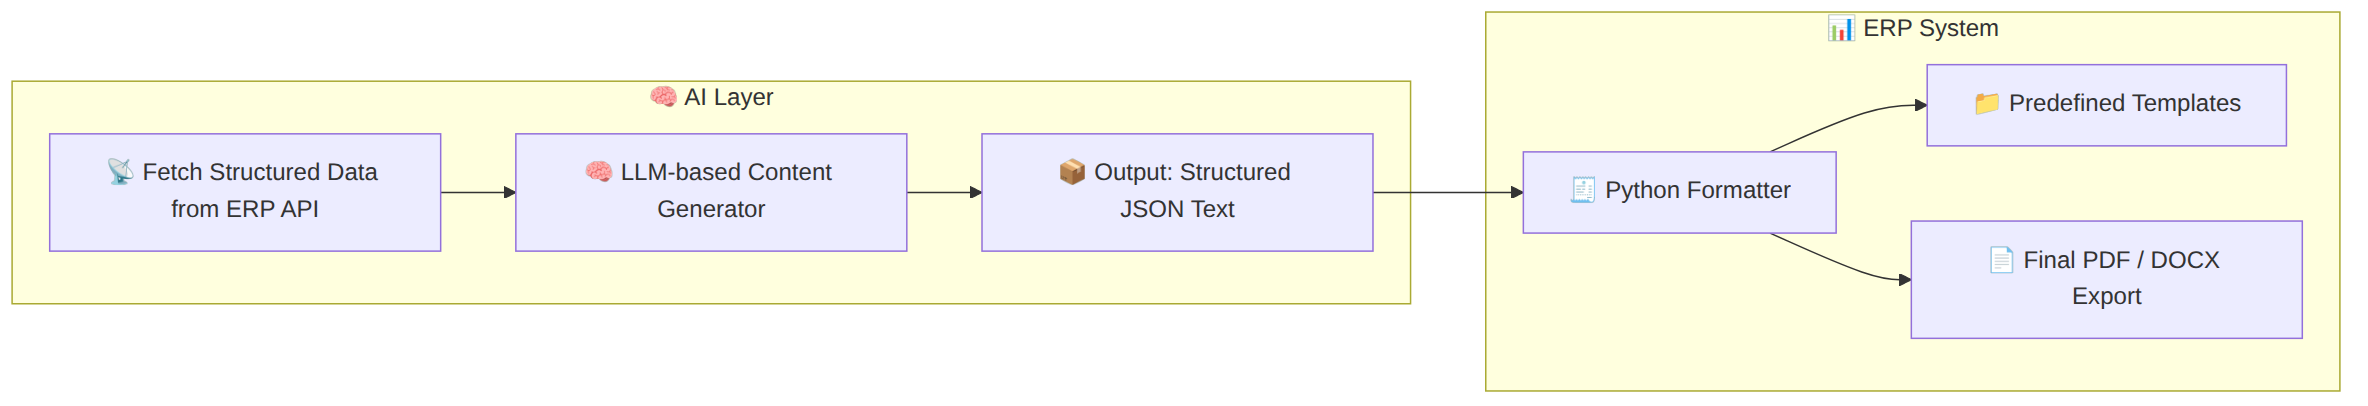
\includegraphics[width=\textwidth,height=0.8\textheight,keepaspectratio]{../../pics/doc-generation.png}
\caption{Document Generation Agent Workflow and AI Layer Integration}
\label{fig:doc-generation-workflow}
\end{figure}

\section{Scope and Boundaries}
\subsection{AI Layer Scope (In-Scope)}
The Document Generation Agent is responsible only for components within the \textbf{AI Layer} subgraph:
\begin{itemize}
  \item \textbf{Data Fetching}: Retrieval of structured data from ERP API endpoints
  \item \textbf{LLM-based Content Generation}: 
    \begin{itemize}
      \item Intelligent narrative text generation
      \item Template content population with contextual information
      \item Dynamic content adaptation based on document type and requirements
    \end{itemize}
  \item \textbf{Structured Output Generation}: Production of organized JSON output containing generated text and structured content
\end{itemize}

\subsection{External Dependencies (Out-of-Scope)}
The following components are \textbf{outside} the AI Layer and handled by the ERP System:
\begin{itemize}
  \item \textbf{ERP Layer Components}:
    \begin{itemize}
      \item Python-based document formatting and layout processing
      \item Predefined template management and selection
      \item Final document export (PDF/DOCX generation)
      \item Document storage and versioning systems
    \end{itemize}
\end{itemize}

\subsection{Integration Boundaries}
\begin{itemize}
  \item \textbf{Input}: Accesses structured data through ERP API interfaces
  \item \textbf{Output}: Delivers structured JSON content to ERP Layer formatting systems
  \item \textbf{Dependencies}: Requires access to project data, templates metadata, and content guidelines
  \item \textbf{Limitations}: Cannot directly control document formatting, template design, or final export processes
\end{itemize}

\section{Architecture Components}
The Document Generation Agent operates exclusively within the AI Layer and consists of the following components:

\subsection{AI Layer Components (Document Generation Agent Scope)}
\begin{itemize}
  \item \textbf{ERP API Interface}: Establishes connections and fetches structured data from various ERP endpoints
  \item \textbf{LLM-based Content Generator}:
    \begin{itemize}
      \item \textbf{Narrative Engine}: Generates contextual descriptions and explanations
      \item \textbf{Template Populator}: Fills template fields with appropriate content
      \item \textbf{Content Adapter}: Adjusts tone, style, and technical level based on document type
    \end{itemize}
  \item \textbf{JSON Formatter}: Structures generated content into organized JSON output for downstream processing
\end{itemize}

\subsection{External Layer Dependencies (Outside AI Agent Scope)}
These components are managed by the ERP System but interface with the AI Layer:
\begin{itemize}
  \item \textbf{Downstream Dependencies}:
    \begin{itemize}
      \item Python Formatter (ERP Layer)
      \item Predefined Templates (ERP Layer)
      \item Document Export System (PDF/DOCX generation)
    \end{itemize}
\end{itemize}

\section{Template Versioning}
To ensure consistent document formats and support rollback:
\begin{itemize}
  \item All templates are stored with semantic version tags in the Knowledge Base (e.g., v1.2.0).
  \item Template updates require a changelog entry and approval before deployment.
  \item The agent selects the template version based on the project’s configuration.
\end{itemize}

\section{Sample Template Snippet}
An example JSON-based template definition:
\begin{lstlisting}[language=JSON]
{
  "templateId": "datasheet_equip_v1",
  "version": "1.2.0",
  "fields": [
    {"name": "equipmentName", "type": "text"},
    {"name": "capacity", "type": "number", "format": "%0.2f"},
    {"name": "operatingTemp", "type": "number", "unit": "\"C\""}
  ],
  "narrativeSections": [
    {"id": "introduction", "prompt": "Generate intro for {{equipmentName}} with capacity {{capacity}}."}
  ],
  "render": {
    "engine": "wkhtmltopdf",
    "options": {"margin-top": "15mm", "margin-bottom": "15mm"}
  }
}
\end{lstlisting}

\section{Document Generation Agent}
\begin{description}
  \item Inputs
    \begin{itemize}
      \item JSON containing:
      \begin{itemize}
        \item \texttt{templateId}
        \item context data fields
      \end{itemize}
    \end{itemize}
  \item Outputs
    \begin{itemize}
      \item Generated document (PDF or Word) as URL or binary payload
    \end{itemize}
  \item Trigger Events
    \begin{itemize}
      \item HTTP POST \texttt{/agents/docgen}
      \item User or workflow-initiated request
    \end{itemize}
  \item External Dependencies / APIs:
    \begin{itemize}
      \item Knowledge Base for template retrieval  
      \item LLM runtime for narrative sections  
      \item Jinja2 (or equivalent) template engine  
      \item Rendering engine (e.g.\ \texttt{wkhtmltopdf})  
      \item File Management API for storing the output document  
    \end{itemize}
\end{description}
\section{Use Case}
A manager requests a compliance certificate for a completed project. The Document Generation Agent:
\begin{enumerate}
  \item Fetches structured project data, compliance results, and specifications from ERP APIs
  \item Uses LLM-based content generation to create narrative sections describing compliance status
  \item Generates contextual explanations for technical parameters and regulatory requirements
  \item Outputs structured JSON containing generated content and data mappings
  \item Passes JSON output to ERP Layer formatting system for final PDF certificate generation
\end{enumerate}

\chapter{Diagram Parsing Agent}
\section{Function}
The Diagram Parsing Agent operates as a specialized AI component that transforms raw P\&ID (Process and Instrumentation Diagram) and CAD files into structured, machine-readable graph representations. It utilizes computer vision, OCR technology, and spatial analysis to identify equipment, extract connectivity information, and build comprehensive network models of industrial processes.

\begin{figure}[htbp]
\centering
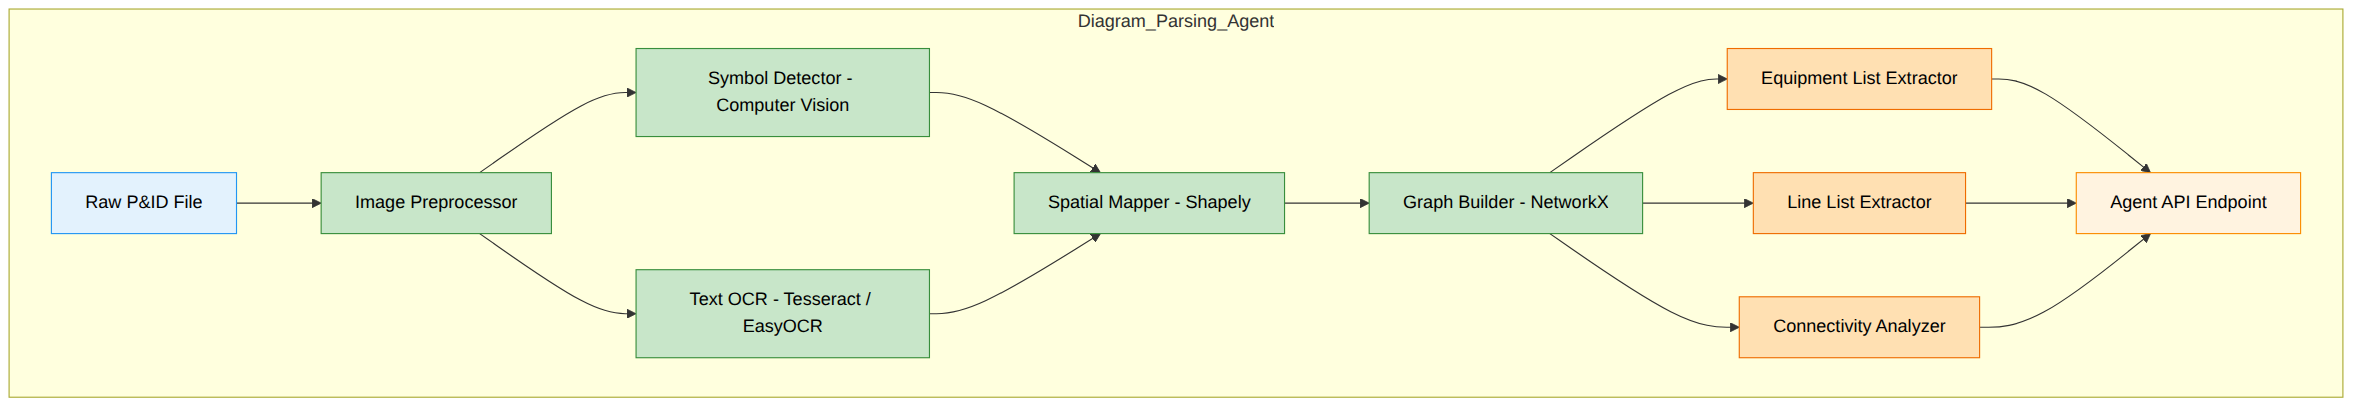
\includegraphics[width=\textwidth,height=1.2\textheight,keepaspectratio]{../../pics/diagram-parser.png}
\caption{Diagram Parsing Agent Processing Pipeline and Component Architecture}
\label{fig:diagram-parser-workflow}
\end{figure}

\section{Scope and Boundaries}
\subsection{Diagram Parsing Agent Scope (In-Scope)}
The Diagram Parsing Agent is responsible for the complete processing pipeline within its component boundary:
\begin{itemize}
  \item \textbf{Image Preprocessing}: 
    \begin{itemize}
      \item Raw P\&ID file ingestion and format normalization
      \item Image enhancement and noise reduction
      \item Resolution optimization for analysis
    \end{itemize}
  \item \textbf{Computer Vision Processing}:
    \begin{itemize}
      \item Symbol detection using advanced computer vision algorithms
      \item Equipment identification and classification
      \item Shape and pattern recognition for industrial symbols
    \end{itemize}
  \item \textbf{Text Recognition and Extraction}:
    \begin{itemize}
      \item OCR using Tesseract/EasyOCR for text extraction
      \item Label identification and association
      \item Tag number and specification text recognition
    \end{itemize}
  \item \textbf{Spatial Analysis and Mapping}:
    \begin{itemize}
      \item Spatial relationship analysis using Shapely
      \item Coordinate mapping and positioning
      \item Connection line detection and tracing
    \end{itemize}
  \item \textbf{Graph Construction}:
    \begin{itemize}
      \item Network graph building using NetworkX
      \item Node and edge relationship establishment
      \item Topology validation and verification
    \end{itemize}
  \item \textbf{Structured Output Generation}:
    \begin{itemize}
      \item Equipment List Extraction with specifications
      \item Line List Extraction with connectivity details
      \item Connectivity Analysis with relationship mapping
    \end{itemize}
  \item \textbf{API Service Integration}:
    \begin{itemize}
      \item RESTful API endpoint provision
      \item JSON output formatting and delivery
      \item Error handling and status reporting
    \end{itemize}
\end{itemize}

\subsection{External Dependencies (Out-of-Scope)}
The following components are outside the Diagram Parsing Agent's direct control:
\begin{itemize}
  \item \textbf{CAD Authoring and Modification}: Cannot create or edit original CAD files
  \item \textbf{File Storage and Management}: Does not handle long-term storage of input or output files
  \item \textbf{Diagram Validation}: Does not verify engineering accuracy or compliance of source diagrams
  \item \textbf{Real-time Collaboration}: Does not support multi-user editing or version control
  \item \textbf{External System Integration}: Direct integration with CAD software or ERP systems beyond API endpoints
\end{itemize}

\subsection{Technical Limitations}
\begin{itemize}
  \item \textbf{Input Format Constraints}: Limited to supported image formats (PDF, PNG, JPEG, TIFF)
  \item \textbf{Diagram Quality Dependencies}: Performance depends on input diagram clarity and resolution
  \item \textbf{Symbol Library Scope}: Recognition limited to trained symbol sets and standard industrial notation
  \item \textbf{Complex Topology Handling}: May require manual validation for highly complex or non-standard layouts
\end{itemize}

\section{Architecture Components}
The Diagram Parsing Agent consists of a comprehensive processing pipeline with specialized components:

\subsection{Core Processing Components}
\begin{itemize}
  \item \textbf{Image Preprocessor}:
    \begin{itemize}
      \item \textbf{Format Handler}: Supports multiple input formats (PDF, PNG, JPEG, TIFF)
      \item \textbf{Enhancement Engine}: Noise reduction, contrast adjustment, resolution optimization
      \item \textbf{Segmentation Module}: Region of interest identification and extraction
    \end{itemize}
  \item \textbf{Symbol Detector (Computer Vision)}:
    \begin{itemize}
      \item \textbf{Pattern Matching}: Template-based symbol recognition
      \item \textbf{Machine Learning Models}: Trained classifiers for equipment identification
      \item \textbf{Confidence Scoring}: Reliability assessment for detected symbols
    \end{itemize}
  \item \textbf{Text OCR Engine}:
    \begin{itemize}
      \item \textbf{Tesseract Integration}: Primary OCR engine for text extraction
      \item \textbf{EasyOCR Support}: Alternative OCR for improved accuracy
      \item \textbf{Text Processing}: Label cleaning, formatting, and association
    \end{itemize}
  \item \textbf{Spatial Mapper}:
    \begin{itemize}
      \item \textbf{Shapely Integration}: Geometric analysis and spatial relationships
      \item \textbf{Coordinate System}: Consistent positioning and measurement
      \item \textbf{Connection Tracing}: Line following and intersection detection
    \end{itemize}
  \item \textbf{Graph Builder}:
    \begin{itemize}
      \item \textbf{NetworkX Integration}: Graph data structure construction
      \item \textbf{Node Management}: Equipment and junction point representation
      \item \textbf{Edge Definition}: Connection and flow relationship establishment
    \end{itemize}
\end{itemize}

\subsection{Output Generation Components}
\begin{itemize}
  \item \textbf{Equipment List Extractor}:
    \begin{itemize}
      \item \textbf{Equipment Catalog}: Comprehensive equipment identification and specification
      \item \textbf{Metadata Association}: Equipment properties, ratings, and characteristics
      \item \textbf{Standardization}: Consistent naming and classification schemes
    \end{itemize}
  \item \textbf{Line List Extractor}:
    \begin{itemize}
      \item \textbf{Piping Identification}: Line routing and specification details
      \item \textbf{Flow Direction}: Process flow analysis and direction determination
      \item \textbf{Material Specifications}: Pipe sizing, materials, and ratings
    \end{itemize}
  \item \textbf{Connectivity Analyzer}:
    \begin{itemize}
      \item \textbf{Topology Mapping}: Complete process flow connectivity
      \item \textbf{Relationship Analysis}: Equipment interdependencies and process relationships
      \item \textbf{Validation Checks}: Connectivity consistency and completeness verification
    \end{itemize}
  \item \textbf{API Endpoint}:
    \begin{itemize}
      \item \textbf{RESTful Interface}: Standard HTTP API for external integration
      \item \textbf{JSON Formatting}: Structured output in JSON format
      \item \textbf{Error Handling}: Comprehensive error reporting and status codes
    \end{itemize}
\end{itemize}

\section{Diagram Parsing Agent}
\begin{description}
  \item Inputs 
    \begin{itemize}
      \item  P\&ID file (PDF, SVG, PNG, JPEG)
    \end{itemize}
  \item Outputs 
    \begin{itemize}
      \item JSON graph including:
      \begin{itemize}
        \item equipment list  
        \item line list  
        \item connectivity data  
      \end{itemize}
    \end{itemize}
  \item Trigger Events
    \begin{itemize}
      \item HTTP POST \texttt{/agents/diagram-parse}
      \item File-upload event from File Management
    \end{itemize}
  \item External Dependencies / APIs:
    \begin{itemize}
      \item OpenCV for symbol detection  
      \item Tesseract or EasyOCR for text extraction  
      \item Shapely for spatial mapping  
      \item NetworkX for graph construction  
      \item Prometheus for performance metrics  
    \end{itemize}
\end{description}

\section{Use Case}
An engineering team uploads a Process Flow Diagram (P\&ID) for a chemical processing unit. The Diagram Parsing Agent:
\begin{enumerate}
  \item \textbf{Receives the P\&ID file}: Ingests the PDF/image file and validates format compatibility
  \item \textbf{Preprocesses the image}: Enhances image quality, adjusts contrast, and optimizes resolution for analysis
  \item \textbf{Detects symbols and equipment}: Uses computer vision to identify pumps, valves, vessels, and instrumentation
  \item \textbf{Extracts text labels}: Applies OCR to extract equipment tags, specifications, and process parameters
  \item \textbf{Maps spatial relationships}: Analyzes the positioning and connections between identified components
  \item \textbf{Builds process graph}: Constructs a NetworkX graph representing the complete process topology
  \item \textbf{Generates structured outputs}:
    \begin{itemize}
      \item Equipment List: JSON array of all identified equipment with tags and specifications
      \item Line List: Comprehensive piping and connection details
      \item Connectivity Analysis: Process flow relationships and interdependencies
    \end{itemize}
  \item \textbf{Delivers via API}: Returns structured JSON data through RESTful API endpoint for integration with downstream systems
\end{enumerate}

\chapter{Email Agent}
\section{Function}
The Email Agent operates within the AI Layer of the system architecture and performs intelligent processing of inbound emails to extract structured information, classify content types, and route processed data to appropriate ERP modules. It utilizes NLP parsing, intent classification, and RAG-based analysis to understand email content and context.

\begin{figure}[htbp]
\centering
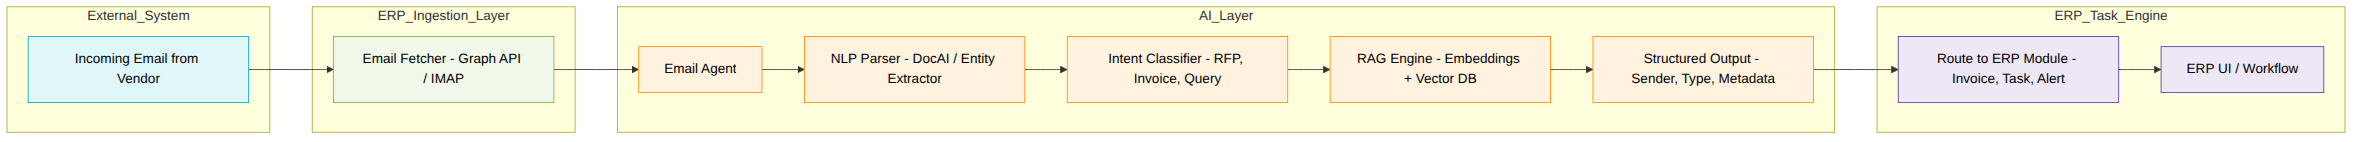
\includegraphics[width=\textwidth,height=1.2\textheight,keepaspectratio]{../../pics/email-agent.png}
\caption{Email Agent Processing Workflow and Layer Integration}
\label{fig:email-agent-workflow}
\end{figure}

\section{Scope and Boundaries}
\subsection{AI Layer Scope (In-Scope)}
The Email Agent is responsible only for components within the \textbf{AI Layer} subgraph:
\begin{itemize}
  \item \textbf{Email Agent Core}: Central orchestration of email processing workflow within AI layer
  \item \textbf{NLP Parsing}:
    \begin{itemize}
      \item DocAI integration for document analysis
      \item Entity extraction from email content and attachments
      \item Natural language understanding of email body text
    \end{itemize}
  \item \textbf{Intent Classification}:
    \begin{itemize}
      \item Email type identification (RFP, Invoice, Query, Instructions)
      \item Content categorization and priority assessment
      \item Context-aware classification using ML models
    \end{itemize}
  \item \textbf{RAG Engine Integration}:
    \begin{itemize}
      \item Embeddings generation for semantic analysis
      \item Vector database queries for context matching
      \item Knowledge retrieval for enhanced understanding
    \end{itemize}
  \item \textbf{Structured Output Generation}:
    \begin{itemize}
      \item Sender identification and metadata extraction
      \item Email type classification results
      \item Structured metadata and parameter extraction
    \end{itemize}
\end{itemize}

\subsection{External Dependencies (Out-of-Scope)}
The following components are \textbf{outside} the AI Layer and handled by other systems:
\begin{itemize}
  \item \textbf{External System}: Incoming emails from vendors, clients, and external sources
  \item \textbf{ERP Ingestion Layer}:
    \begin{itemize}
      \item Email fetching services (Graph API/IMAP connectivity)
      \item Email server authentication and connection management
      \item Raw email retrieval and initial processing
    \end{itemize}
  \item \textbf{ERP Task Engine}:
    \begin{itemize}
      \item Routing to appropriate ERP modules (Invoice, Task, Alert systems)
      \item ERP UI and workflow integration
      \item Email delivery and notification systems
      \item Task creation and assignment workflows
    \end{itemize}
\end{itemize}

\subsection{Integration Boundaries}
\begin{itemize}
  \item \textbf{Input}: Receives structured email data from ERP Ingestion Layer
  \item \textbf{Output}: Delivers processed email metadata and classification to ERP Task Engine
  \item \textbf{Dependencies}: Accesses shared knowledge bases and vector databases for context
  \item \textbf{Limitations}: Cannot fetch emails directly, deliver responses, or create ERP tasks
\end{itemize}

\section{Architecture Components}
The Email Agent operates exclusively within the AI Layer and consists of the following components:

\subsection{AI Layer Components (Email Agent Scope)}
\begin{itemize}
  \item \textbf{Email Agent Core}:
    \begin{itemize}
      \item \textbf{Workflow Orchestrator}: Manages the email processing pipeline
      \item \textbf{Context Manager}: Maintains email processing state and history
    \end{itemize}
  \item \textbf{NLP Parser}:
    \begin{itemize}
      \item \textbf{DocAI Integration}: Processes attachments and document content
      \item \textbf{Entity Extractor}: Identifies key entities, parameters, and values
      \item \textbf{Text Analyzer}: Processes email body content and metadata
    \end{itemize}
  \item \textbf{Intent Classifier}:
    \begin{itemize}
      \item \textbf{Content Categorizer}: Classifies emails as RFP, Invoice, Query, etc.
      \item \textbf{Priority Assessor}: Determines urgency and importance levels
      \item \textbf{Context Analyzer}: Understands business context and relationships
    \end{itemize}
  \item \textbf{RAG Engine}:
    \begin{itemize}
      \item \textbf{Embedding Generator}: Creates semantic representations of email content
      \item \textbf{Vector Search}: Queries knowledge base for relevant context
      \item \textbf{Knowledge Retriever}: Accesses historical and reference information
    \end{itemize}
  \item \textbf{Output Formatter}:
    \begin{itemize}
      \item \textbf{Metadata Extractor}: Structures sender, recipient, and timing information
      \item \textbf{Classification Reporter}: Provides content type and confidence scores
      \item \textbf{Parameter Organizer}: Formats extracted parameters and instructions
    \end{itemize}
\end{itemize}

\subsection{External Layer Dependencies (Outside AI Agent Scope)}
These components are managed by other systems but interface with the AI Layer:
\begin{itemize}
  \item \textbf{Upstream Dependencies}:
    \begin{itemize}
      \item Email Fetcher services (ERP Ingestion Layer)
      \item External email systems and vendors
    \end{itemize}
  \item \textbf{Downstream Dependencies}:
    \begin{itemize}
      \item ERP Module Router (ERP Task Engine)
      \item ERP UI and workflow systems
    \end{itemize}
\end{itemize}

\section{Email Agent}
\begin{description}
  \item Inputs 
    \begin{itemize}
      \item Raw MIME email (headers, body, attachments)
    \end{itemize}
  \item Outputs
    \begin{itemize}
      \item JSON containing:
      \begin{itemize}
        \item extracted instructions  
        \item parameter values  
        \item attachment metadata  
      \end{itemize}
    \end{itemize}
  \item Trigger Events 
    \begin{itemize}
      \item HTTP POST \texttt{/agents/email-parse}
      \item Incoming email webhook  
    \end{itemize}
  \item External Dependencies / APIs
    \begin{itemize}
      \item MIME parsing library (e.g.\ Python \texttt{email}, MimeKit)  
      \item LLM runtime for intent detection  
      \item Virus-scan service for attachments  
      \item Prometheus metrics endpoint  
    \end{itemize}
\end{description}

\section{Use Case}
A vendor sends an email with subject ``Run simulation at 6 bar pressure for Project Alpha'' with P\&ID attachments. The Email Agent:
\begin{enumerate}
  \item Receives structured email data from the ERP Ingestion Layer email fetcher
  \item Uses NLP parser with DocAI to extract text from email body and analyze P\&ID attachments
  \item Identifies entities: ``simulation'', ``6 bar pressure'', ``Project Alpha''
  \item Classifies the email intent as ``Instruction/Task Request'' using the intent classifier
  \item Applies RAG engine to match against similar historical requests and project context
  \item Generates structured output with sender metadata, classification (Instruction), and extracted parameters
  \item Delivers structured output to ERP Task Engine for routing to appropriate project management module
\end{enumerate}

\chapter{ERP-Chat Agent}
\section{Function}
The ERP-Chat Agent operates within the AI Layer of the system architecture and provides intelligent natural language interface for querying ERP systems. It processes user queries through natural language understanding, semantic analysis, and API routing to deliver structured responses about equipment, project data, and system information.

\begin{figure}[htbp]
\centering
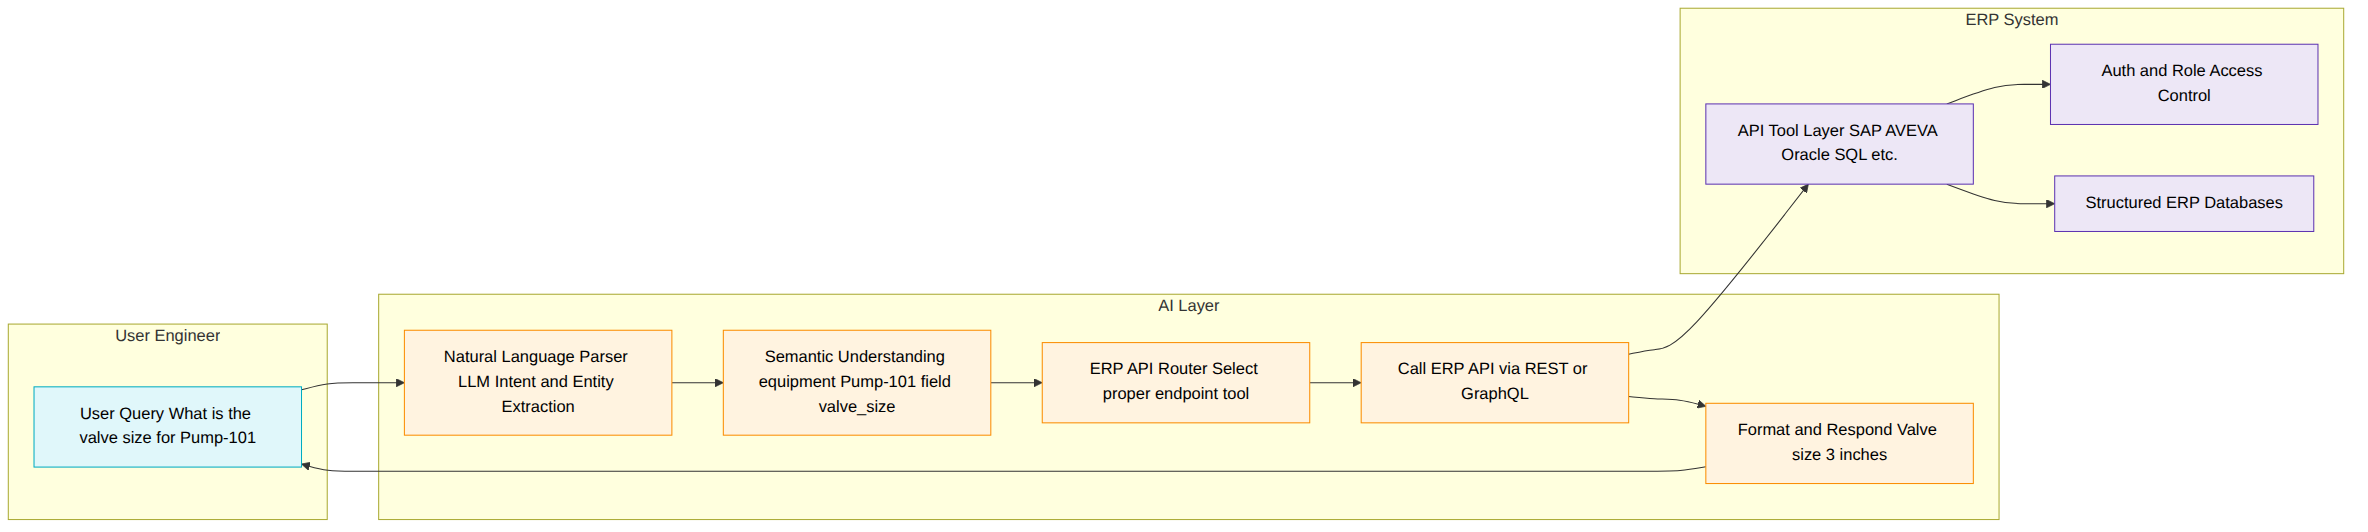
\includegraphics[width=\textwidth,height=0.8\textheight,keepaspectratio]{../../pics/erp-chat.png}
\caption{ERP-Chat Agent Natural Language Processing and API Integration}
\label{fig:erp-chat-workflow}
\end{figure}

\section{Scope and Boundaries}
\subsection{AI Layer Scope (In-Scope)}
The ERP-Chat Agent is responsible only for components within the \textbf{AI Layer} subgraph:
\begin{itemize}
  \item \textbf{Natural Language Processing}: 
    \begin{itemize}
      \item LLM-based intent extraction from user queries
      \item Entity recognition and parameter identification
      \item Context understanding and query disambiguation
    \end{itemize}
  \item \textbf{Semantic Understanding}:
    \begin{itemize}
      \item Equipment identification and mapping (e.g., Pump-101 to valve\_size field)
      \item Relationship analysis between entities and attributes
      \item Domain-specific terminology interpretation
    \end{itemize}
  \item \textbf{ERP API Routing}:
    \begin{itemize}
      \item Selection of appropriate API endpoints and tools
      \item Query translation to API-compatible formats
      \item REST/GraphQL call preparation
    \end{itemize}
  \item \textbf{Response Formatting}:
    \begin{itemize}
      \item Natural language response generation
      \item Context-aware answer formatting
      \item User-friendly presentation of technical data
    \end{itemize}
\end{itemize}

\subsection{External Dependencies (Out-of-Scope)}
The following components are \textbf{outside} the AI Layer and handled by other systems:
\begin{itemize}
  \item \textbf{User Interface}: External user interaction systems and chat interfaces
  \item \textbf{ERP System Components}:
    \begin{itemize}
      \item API Tool Layer (SAP, AVEVA, Oracle, SQL databases)
      \item Authentication and Role-based Access Control
      \item Structured ERP databases and data storage
      \item Task orchestration and workflow management logic
    \end{itemize}
\end{itemize}

\subsection{Integration Boundaries}
\begin{itemize}
  \item \textbf{Input}: Receives natural language queries from external user interfaces
  \item \textbf{Output}: Delivers formatted natural language responses to users
  \item \textbf{Dependencies}: Accesses ERP APIs through secure authentication layers
  \item \textbf{Limitations}: Cannot modify ERP data, create tasks, or perform administrative actions beyond read queries
\end{itemize}

\section{Architecture Components}
The ERP-Chat Agent operates exclusively within the AI Layer and consists of the following components:

\subsection{AI Layer Components (ERP-Chat Agent Scope)}
\begin{itemize}
  \item \textbf{Natural Language Parser}:
    \begin{itemize}
      \item \textbf{Intent Extraction}: Identifies user query objectives and goals
      \item \textbf{Entity Recognition}: Extracts equipment names, parameters, and values
      \item \textbf{Context Manager}: Maintains conversation context and query history
    \end{itemize}
  \item \textbf{Semantic Understanding Engine}:
    \begin{itemize}
      \item \textbf{Equipment Mapper}: Links natural language references to ERP entities
      \item \textbf{Field Resolver}: Maps requested information to database fields
      \item \textbf{Relationship Analyzer}: Understands equipment hierarchies and dependencies
    \end{itemize}
  \item \textbf{ERP API Router}:
    \begin{itemize}
      \item \textbf{Endpoint Selector}: Chooses appropriate API tools and endpoints
      \item \textbf{Query Builder}: Constructs REST/GraphQL queries
      \item \textbf{Response Handler}: Processes API responses and error handling
    \end{itemize}
  \item \textbf{Response Formatter}:
    \begin{itemize}
      \item \textbf{Natural Language Generator}: Creates human-readable responses
      \item \textbf{Data Presenter}: Formats technical information appropriately
      \item \textbf{Context Integrator}: Includes relevant context in responses
    \end{itemize}
\end{itemize}

\subsection{External Layer Dependencies (Outside AI Agent Scope)}
These components are managed by other systems but interface with the AI Layer:
\begin{itemize}
  \item \textbf{Upstream Dependencies}:
    \begin{itemize}
      \item User interface systems and chat platforms
    \end{itemize}
  \item \textbf{Downstream Dependencies}:
    \begin{itemize}
      \item ERP API Tool Layer (SAP, AVEVA, Oracle, SQL)
      \item Authentication and Access Control systems
      \item ERP databases and data repositories
    \end{itemize}
\end{itemize}

\section{ERP Action Agent}
\begin{description}
  \item Inputs
    \begin{itemize}
      \item Natural-language command  
      \item Project context  
      \item JWT authentication token  
    \end{itemize}
  \item Outputs
    \begin{itemize}
      \item Confirmation JSON containing:
      \begin{itemize}
        \item \texttt{taskId}  
        \item status message  
      \end{itemize}
    \end{itemize}
  \item Trigger Events
    \begin{itemize}
      \item HTTP POST \texttt{/agents/erp-action}
      \item Chatbot or CLI command  
    \end{itemize}
  \item External Dependencies / APIs
    \begin{itemize}
      \item ERP Task Engine REST API  
      \item JSON Schema validator  
      \item LLM runtime for NL-to-API mapping  
      \item Prometheus \& Loki for logging  
    \end{itemize}
\end{description}

\section{Use Case}
A user asks: ``What is the valve size for Pump-101?'' The ERP-Chat Agent:
\begin{enumerate}
  \item Parses the natural language query using LLM for intent and entity extraction
  \item Identifies ``Pump-101'' as equipment entity and ``valve size'' as the requested field
  \item Uses semantic understanding to map the query to appropriate ERP database fields
  \item Routes the query to the correct ERP API endpoint with proper authentication
  \item Calls the ERP API via REST/GraphQL to retrieve the valve size information
  \item Formats the response into natural language: ``Valve size: 3 inches''
  \item Delivers the formatted response back to the user
\end{enumerate}

\chapter{Shared Services and Infrastructure}
\section{Infrastructure Architecture Overview}
The AI Agent Module is built on a robust, scalable infrastructure architecture that leverages microservices patterns, containerization, and Infrastructure as Code (IaC) principles. This chapter details the comprehensive infrastructure design, deployment strategy, and architectural decisions that enable high availability, scalability, and maintainability.



\section{Kubernetes Architecture}
The system leverages Kubernetes orchestration to provide container management, service discovery, and automated scaling capabilities.

\begin{figure}[htbp]
\centering
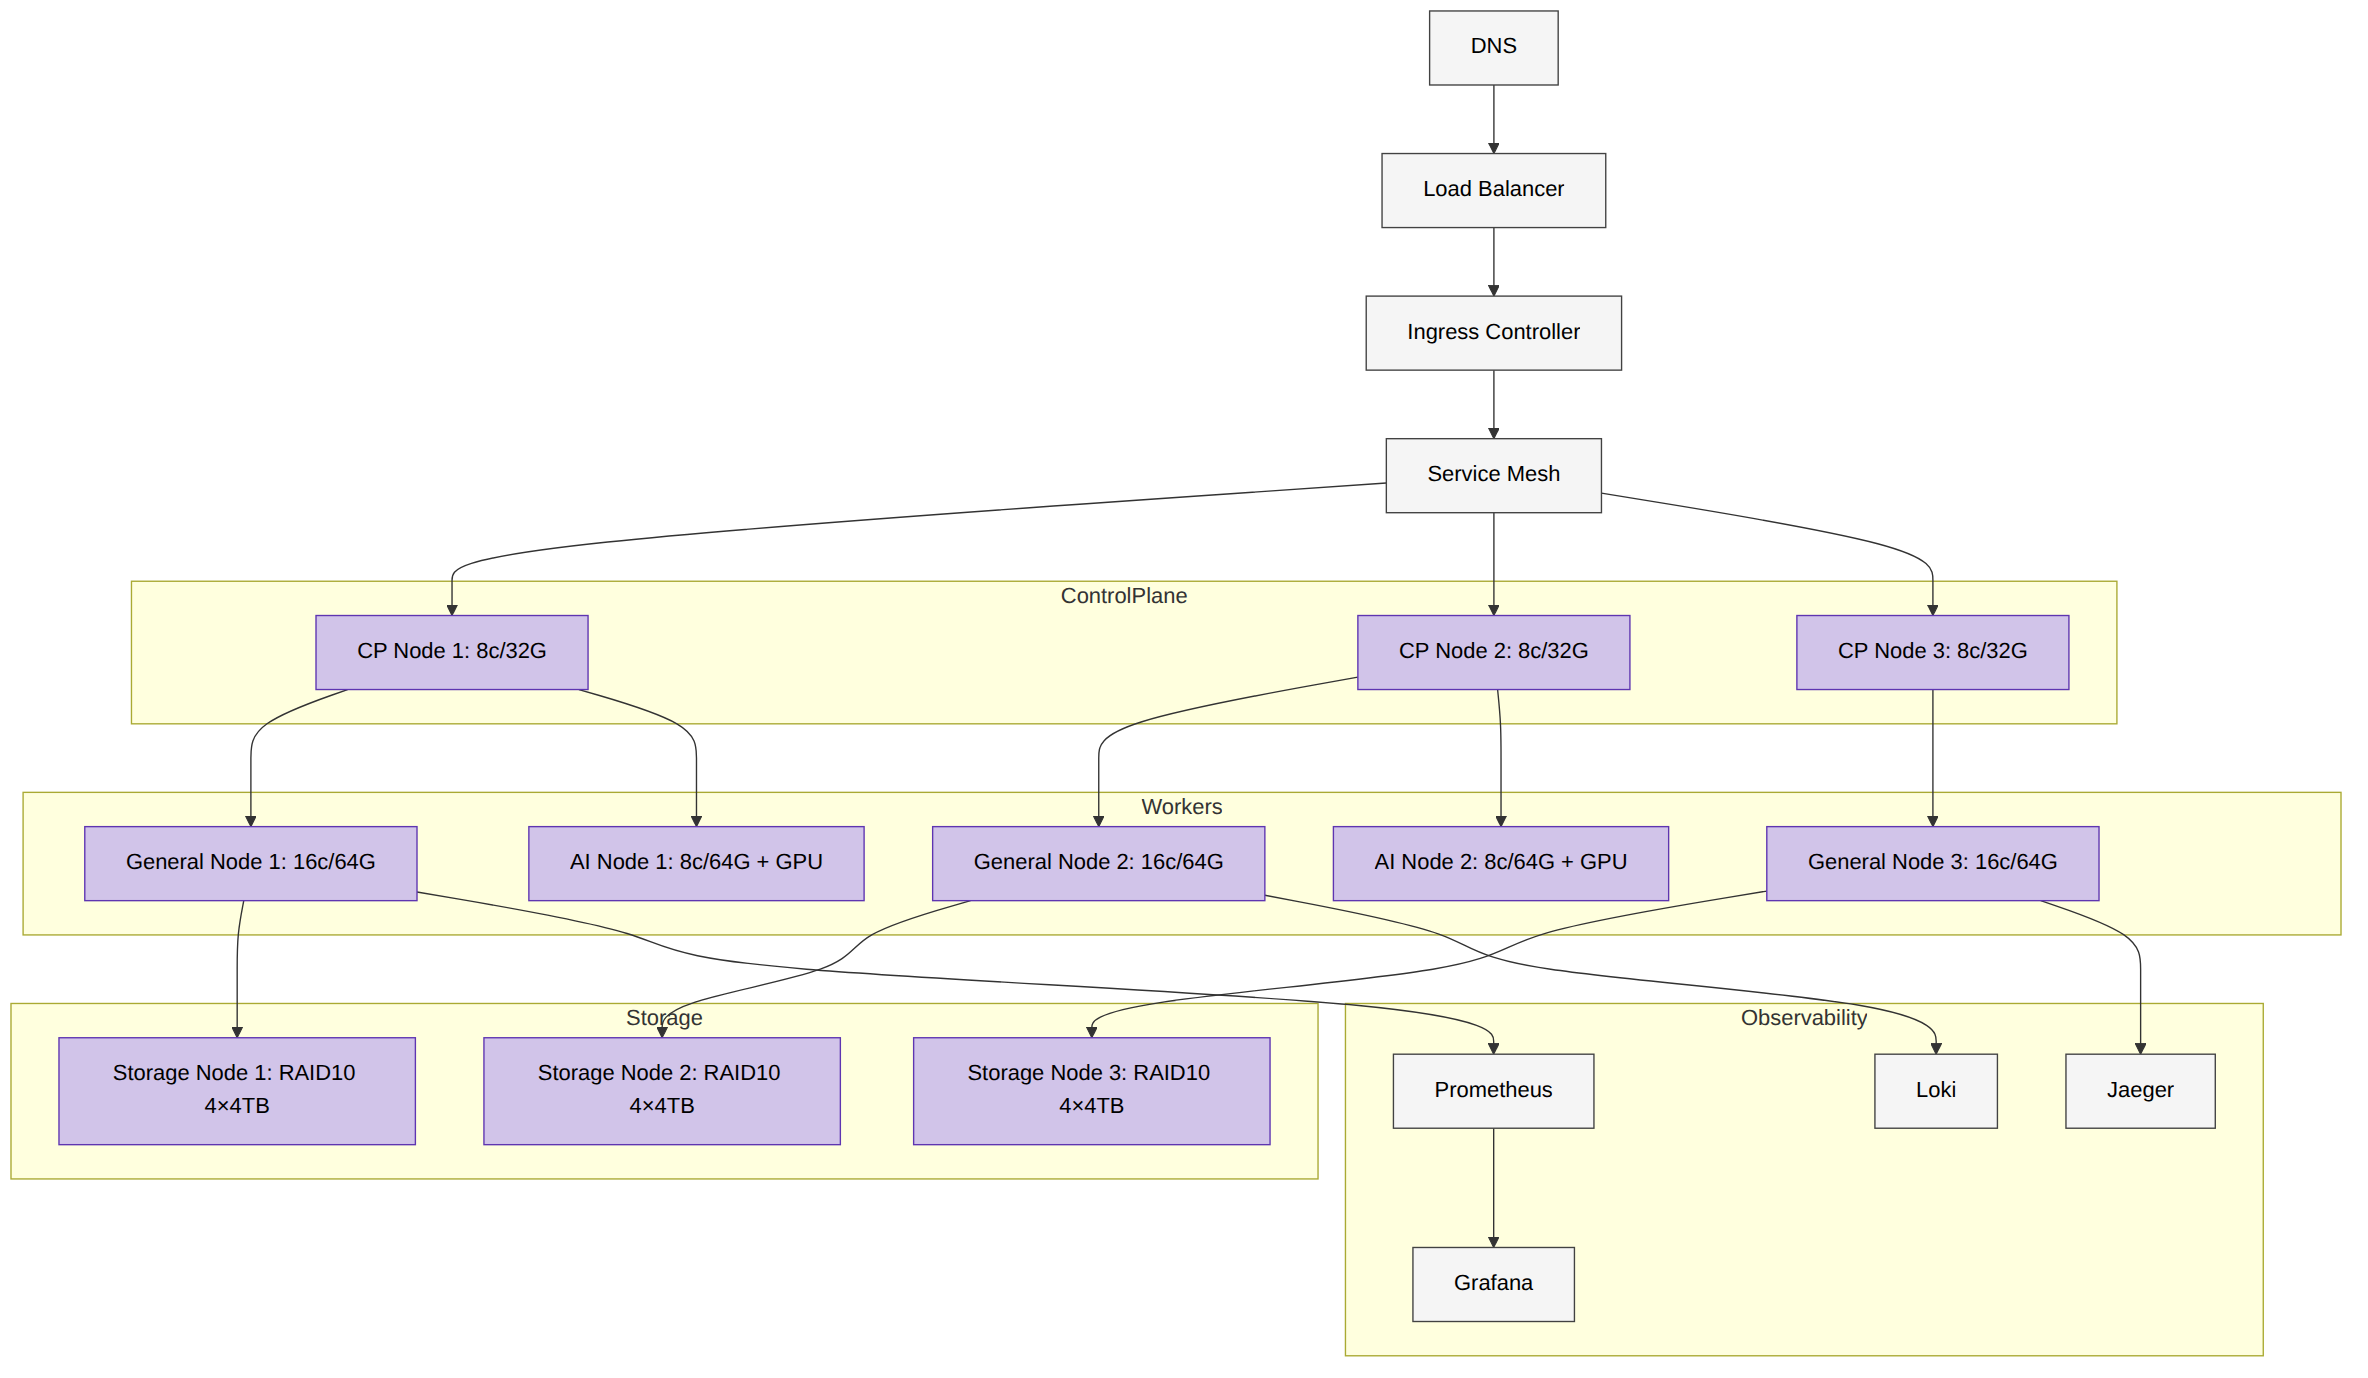
\includegraphics[width=\textwidth,height=0.8\textheight,keepaspectratio]{../../pics/arch.png}
\caption{Kubernetes Cluster Architecture and Service Topology}
\label{fig:k8s-architecture}
\end{figure}

\subsection{Network and Ingress Layer}
\begin{itemize}
  \item \textbf{DNS Resolution}: External DNS routing to load balancer
  \item \textbf{Load Balancer}: High-availability traffic distribution
  \item \textbf{Ingress Controller}: Kubernetes-native traffic routing and SSL termination
  \item \textbf{Service Mesh}: Inter-service communication, security, and observability
\end{itemize}

\subsection{Control Plane Configuration}
\begin{itemize}
  \item \textbf{High Availability}: 3-node control plane with etcd clustering
  \item \textbf{API Server}: RESTful API for cluster management
  \item \textbf{Scheduler}: Intelligent workload placement across nodes
  \item \textbf{Controller Manager}: Automated cluster state management
\end{itemize}

\subsection{Worker Node Specialization}
\begin{itemize}
  \item \textbf{General Workers}: Application services, API gateways, business logic
  \item \textbf{AI Workers}: GPU-accelerated nodes for machine learning workloads
  \item \textbf{Storage Workers}: Persistent volume hosting and data services
\end{itemize}

\section{Microservices Architecture Benefits}

\subsection{Scalability and Performance}
\begin{itemize}
  \item \textbf{Independent Scaling}: Each AI agent can scale based on demand
  \item \textbf{Resource Optimization}: GPU resources allocated only to AI workloads
  \item \textbf{Load Distribution}: Workloads distributed across specialized nodes
  \item \textbf{Horizontal Scaling}: Add more instances of high-demand services
\end{itemize}

\subsection{Development and Deployment Agility}
\begin{itemize}
  \item \textbf{Independent Development}: Teams can develop agents independently
  \item \textbf{Technology Diversity}: Different agents can use optimal technology stacks
  \item \textbf{Rapid Deployment}: Individual service updates without system-wide impact
  \item \textbf{Rolling Updates}: Zero-downtime deployments with gradual rollouts
\end{itemize}

\subsection{Fault Isolation and Resilience}
\begin{itemize}
  \item \textbf{Failure Containment}: Agent failures don't cascade to other services
  \item \textbf{Circuit Breakers}: Automatic failure detection and recovery
  \item \textbf{Redundancy}: Multiple instances provide fault tolerance
  \item \textbf{Health Monitoring}: Proactive issue detection and resolution
\end{itemize}

\subsection{Maintainability and Testing}
\begin{itemize}
  \item \textbf{Modular Architecture}: Clear separation of concerns and responsibilities
  \item \textbf{Independent Testing}: Unit and integration testing per service
  \item \textbf{Version Management}: Independent versioning and compatibility
  \item \textbf{Code Ownership}: Clear responsibility boundaries for teams
\end{itemize}

\section{Infrastructure as Code (IaC) Implementation}

\subsection{IaC Advantages and Benefits}
\begin{itemize}
  \item \textbf{Reproducibility}: Consistent environment creation across development, staging, and production
  \item \textbf{Version Control}: Infrastructure changes tracked in Git with full audit trail
  \item \textbf{Automated Deployment}: Eliminate manual configuration errors and reduce deployment time
  \item \textbf{Disaster Recovery}: Rapid environment reconstruction from code definitions
  \item \textbf{Cost Management}: Resource optimization through programmatic resource allocation
  \item \textbf{Compliance}: Automated compliance checks and policy enforcement
\end{itemize}

\subsection{IaC Technology Stack}
\begin{itemize}
  \item \textbf{Terraform}: Infrastructure provisioning and resource management
  \item \textbf{Ansible}: Configuration management and application deployment
  \item \textbf{Helm Charts}: Kubernetes application packaging and templating
  \item \textbf{GitOps}: Git-based deployment workflows with ArgoCD/Flux
\end{itemize}

\subsection{IaC Implementation Strategy}
\begin{itemize}
  \item \textbf{Modular Design}: Reusable infrastructure components and templates
  \item \textbf{Environment Separation}: Distinct configurations for dev/staging/production
  \item \textbf{State Management}: Centralized state storage with locking mechanisms
  \item \textbf{Change Validation}: Automated testing and validation pipelines
\end{itemize}

\section{Core Infrastructure Services}

\subsection{LLM Runtime}
\begin{itemize}
  \item \textbf{Architecture}: Hosted on dedicated GPU nodes via Kubernetes
  \item \textbf{Resource Allocation}: Tesla T4 GPUs with 128GB RAM per node
  \item \textbf{Model Management}: Containerized model serving with version control
  \item \textbf{Load Balancing}: Automatic request distribution across GPU nodes
  \item \textbf{Scaling Strategy}: Horizontal Pod Autoscaler based on GPU utilization
\end{itemize}

\subsection{Embedding Service and Vector Database}
\begin{itemize}
  \item \textbf{Technology Stack}: Faiss/Qdrant for semantic retrieval operations
  \item \textbf{Data Partitioning}: Project-scoped collections for data isolation
  \item \textbf{Performance Optimization}: In-memory indexing with persistent storage
  \item \textbf{Backup Strategy}: Automated vector index backup and restoration
  \item \textbf{Query Optimization}: Efficient similarity search with caching layers
\end{itemize}

\subsection{Knowledge Base}
\begin{itemize}
  \item \textbf{Database Technology}: MongoDB collections scoped by project
  \item \textbf{Data Architecture}: Document-oriented storage for flexible schemas
  \item \textbf{Replication}: 3-node replica sets for high availability
  \item \textbf{Indexing Strategy}: Optimized indexes for query performance
  \item \textbf{Data Governance}: Role-based access control and audit logging
\end{itemize}

\subsection{Message Queue}
\begin{itemize}
  \item \textbf{Technology}: Apache Kafka topics for agent requests and retries
  \item \textbf{Partitioning Strategy}: Topic partitioning for parallel processing
  \item \textbf{Durability}: Persistent message storage with configurable retention
  \item \textbf{Consumer Groups}: Load distribution across multiple agent instances
  \item \textbf{Dead Letter Queues}: Failed message handling and retry mechanisms
\end{itemize}

\subsection{Observability and Monitoring}
\begin{itemize}
  \item \textbf{Metrics Collection}: Prometheus counters and custom metrics
  \item \textbf{Log Aggregation}: Loki log ingestion with structured logging
  \item \textbf{Distributed Tracing}: Jaeger for request flow analysis
  \item \textbf{Visualization}: Grafana dashboards for operational insights
  \item \textbf{Alerting}: PrometheusAlert manager for incident response
\end{itemize}

\section{Security and Compliance}

\subsection{Container Security}
\begin{itemize}
  \item \textbf{Image Scanning}: Automated vulnerability assessment
  \item \textbf{Runtime Security}: Pod security policies and admission controllers
  \item \textbf{Network Policies}: Micro-segmentation and traffic isolation
  \item \textbf{Secret Management}: Kubernetes secrets with external secret operators
\end{itemize}

\subsection{Authentication and Authorization}
\begin{itemize}
  \item \textbf{Identity Provider}: Integrated OIDC/SAML authentication
  \item \textbf{RBAC}: Kubernetes role-based access control
  \item \textbf{Service Authentication}: mTLS for inter-service communication
  \item \textbf{API Security}: OAuth 2.0/JWT token validation
\end{itemize}

\section{Operational Excellence}

\subsection{Deployment Strategy}
\begin{itemize}
  \item \textbf{CI/CD Pipelines}: Automated testing and deployment workflows
  \item \textbf{Blue-Green Deployments}: Zero-downtime production updates
  \item \textbf{Canary Releases}: Gradual rollouts with automated rollback
  \item \textbf{Feature Flags}: Runtime feature control and A/B testing
\end{itemize}

\subsection{Backup and Disaster Recovery}
\begin{itemize}
  \item \textbf{Data Backup}: Automated database and persistent volume backups
  \item \textbf{Cross-Region Replication}: Geographic redundancy for critical data
  \item \textbf{Recovery Testing}: Regular disaster recovery drills
  \item \textbf{RTO/RPO Goals}: 15-minute Recovery Time/Point Objectives
\end{itemize}

\chapter{Deployment and Operations}
\section{Deployment Strategy}
The deployment strategy follows a robust CI/CD pipeline leveraging GitOps principles to ensure consistent, repeatable deployments across environments. The pipeline includes automated testing, security scanning, and approval gates to maintain high quality and compliance standards.
\subsection{CI/CD Pipeline Stages}
\begin{itemize}
  \item \textbf{Source Control}: Git repository for version control and collaboration
  \item \textbf{Build Stage}: Automated builds with Docker images for each service
  \item \textbf{Test Stage}: Unit, integration, and end-to-end tests
  \item \textbf{Security Scanning}: Automated vulnerability scanning of container images
  \item \textbf{Staging Deployment}: Deploy to staging environment for validation
  \item \textbf{Approval Gates}: Manual review and approval for production deployment
  \item \textbf{Production Deployment}: Automated deployment to production cluster
  \item \textbf{Monitoring and Rollback}: Post-deployment monitoring with automated rollback
\end{itemize}   

\section{Operational Monitoring}
Operational monitoring is critical for maintaining system health and performance. The observability stack includes:
\begin{itemize}
  \item \textbf{Metrics Collection}: Prometheus for real-time metrics and alerting
  \item \textbf{Log Aggregation}: Loki for structured log storage and querying
  \item \textbf{Distributed Tracing}: Jaeger for end-to-end request tracing
  \item \textbf{Dashboards}: Grafana for visualizing metrics, logs, and traces
  \item \textbf{Alerting}: Prometheus Alertmanager for incident response
\end{itemize}
\section{Incident Management}
Incident management processes are established to ensure rapid response and resolution of operational issues. The process includes:
\begin{itemize}
  \item \textbf{Incident Detection}: Automated alerts from monitoring systems
  \item \textbf{Incident Triage}: Initial assessment and categorization of incidents
  \item \textbf{Incident Response Team}: Designated team for incident resolution
  \item \textbf{Root Cause Analysis}: Post-incident review to identify underlying issues
  \item \textbf{Incident Reporting}: Documentation of incidents and resolutions for future reference
\end{itemize}   
\section{Backup and Disaster Recovery}
Backup and disaster recovery strategies are highly relevant for on-premise deployments, as they ensure data integrity and service availability in the event of hardware failures, site outages, or other disruptions. For on-premise environments, it is critical to implement:

\begin{itemize}
    \item \textbf{Automated Backups}: Schedule regular backups of all databases and persistent volumes to local and, if possible, offsite storage.
    \item \textbf{Cross-Site Replication}: If multiple physical locations are available, replicate critical data to a secondary site for geographic redundancy.
    \item \textbf{Disaster Recovery Drills}: Regularly test recovery procedures to validate backup integrity and team readiness.
    \item \textbf{Recovery Time Objectives (RTO)}: Define and monitor RTOs (e.g., 15 minutes for critical services) to ensure rapid restoration.
    \item \textbf{Recovery Point Objectives (RPO)}: Set RPOs (e.g., 15 minutes for critical data) to minimize data loss in case of failure.
    \item \textbf{Offsite Backup Storage}: Use secure, encrypted offsite or cloud storage for backup copies if regulatory and security policies permit.
\end{itemize}

\section{Security and Compliance}
Security and compliance are paramount in the AI Agent Module. As the AI Agent Module is a subsystem within the larger ERP system, core responsibilities such as authentication, authorization, and RBAC are managed by the ERP platform. The AI subsystem enforces the following measures within its scope:
\begin{itemize}
    \item \textbf{Container Security}: Image scanning, runtime security policies, and network segmentation
    \item \textbf{Service Communication Security}: mTLS for secure inter-service communication within the AI subsystem
    \item \textbf{Data Encryption}: Encryption at rest and in transit for sensitive data handled by the AI module
    \item \textbf{Compliance Audits}: Regular security audits and vulnerability assessments for AI-specific components
    \item \textbf{Incident Response Plan}: Established procedures for handling security incidents and breaches within the AI subsystem
\end{itemize}
\textit{Note: All user authentication, authorization, and RBAC enforcement are handled by the ERP system. The AI Agent Module relies on the ERP for identity and access management.}

\chapter{Hardware and Software Requirements}
\section{Hardware Requirements}
The AI Agent Module requires a robust hardware infrastructure to support its computational and storage needs. The infrastructure is designed to run on a single physical host with virtualized components to provide isolation, resource management, and scalability.

\begin{figure}[htbp]
\centering
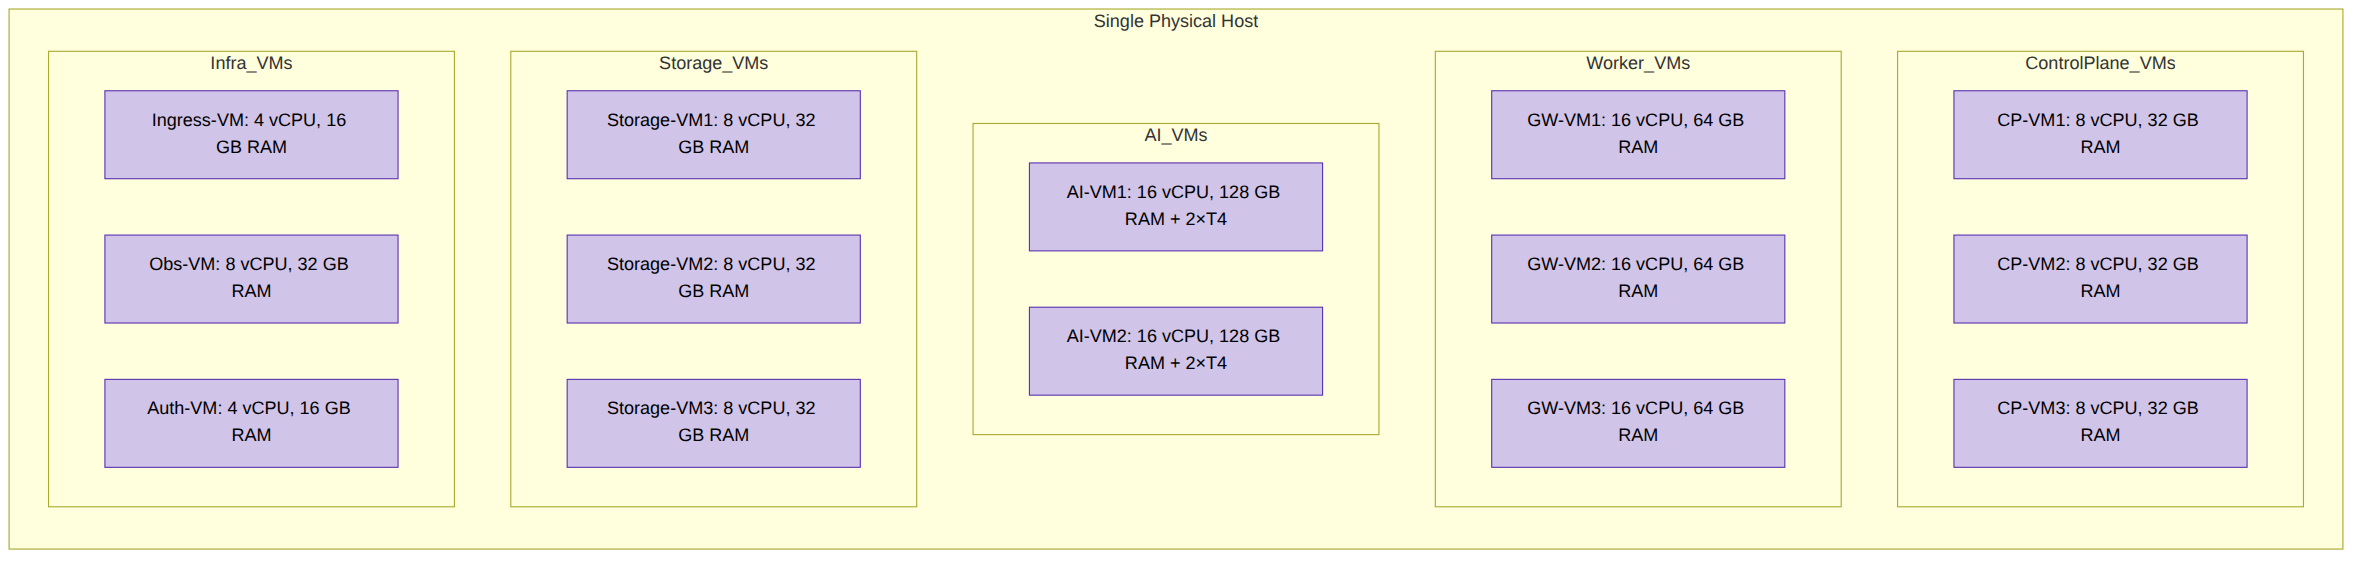
\includegraphics[width=\textwidth,height=0.8\textheight,keepaspectratio]{../../pics/Infra.png}
\caption{Physical Host VM Distribution and Resource Allocation}
\label{fig:server-architecture}
\end{figure}

\subsection{VM Distribution Strategy}
The physical host is divided into specialized virtual machine pools, each optimized for specific workload types:

\subsubsection{Control Plane VMs}
\begin{itemize}
  \item \textbf{Configuration}: 3 VMs × (8 vCPU, 32 GB RAM)
  \item \textbf{Purpose}: Kubernetes control plane management, API server, etcd, scheduler
  \item \textbf{High Availability}: Triple redundancy ensures cluster availability during node failures
  \item \textbf{Resource Optimization}: Moderate CPU/RAM allocation focused on management overhead
\end{itemize}

\subsubsection{General Worker VMs}
\begin{itemize}
  \item \textbf{Configuration}: 3 VMs × (16 vCPU, 64 GB RAM)
  \item \textbf{Purpose}: General application workloads, API gateways, business logic services
  \item \textbf{Scalability}: Higher CPU/RAM allocation for compute-intensive tasks
  \item \textbf{Load Distribution}: Distributed scheduling across multiple nodes
\end{itemize}

\subsubsection{AI-Specialized VMs}
\begin{itemize}
  \item \textbf{Configuration}: 2 VMs × (16 vCPU, 128 GB RAM + 2×T4 GPUs)
  \item \textbf{Purpose}: LLM runtime, embedding generation, AI model inference
  \item \textbf{GPU Acceleration}: Dedicated Tesla T4 GPUs for AI workloads
  \item \textbf{Memory Optimization}: High RAM allocation for large model loading
\end{itemize}

\subsubsection{Storage VMs}
\begin{itemize}
  \item \textbf{Configuration}: 3 VMs × (8 vCPU, 32 GB RAM)
  \item \textbf{Purpose}: Distributed storage, database hosting, persistent volumes
  \item \textbf{Data Redundancy}: Triple replication for data durability
  \item \textbf{I/O Optimization}: Optimized for storage operations and data access
\end{itemize}

\subsubsection{Infrastructure Support VMs}
\begin{itemize}
  \item \textbf{Ingress VM}: 4 vCPU, 16 GB RAM -- Load balancing and traffic routing
  \item \textbf{Observability VM}: 8 vCPU, 32 GB RAM -- Monitoring, logging, and metrics
  \item \textbf{Authentication VM}: 4 vCPU, 16 GB RAM -- Identity and access management
\end{itemize}

\section{Server Specifications and Expected Pricing}
\begin{table}[H]
  \centering
  \footnotesize
  \setlength{\tabcolsep}{2pt} % Reduce column padding
  \begin{tabular}{@{} l c r r l @{}}
    \toprule
    \textbf{Component} & \textbf{Qty} & \textbf{Unit Cost (INR)} & \textbf{Total (INR)} & \textbf{Notes} \\
    \midrule
    Intel Xeon Gold 6348 CPU         & 2  & 573,750 & 1,147,500 & RCP 3,072 × 83/USD \\
    32 GB DDR4 ECC RDIMM             & 16 & 45,000  & 720,000   & 20 K per 32 GB module \\
    NVIDIA Tesla T4 16 GB GPU        & 4  & 325,506 & 1,302,021 & ServerBasket list price \\
    1 TB NVMe SSD (enterprise)       & 4  & 27,000  & 108,000   & ~12 K/TB \\
    8 TB HDD (enterprise, RAID-10)   & 12 & 45,000  & 540,000   & ~20 K each \\
    Dual-port 25 GbE NIC             & 2  & 56,250  & 112,500   & SFP28 cards \\
    Dual-port 10 GbE NIC             & 2  & 27,000  & 54,000    & SFP+ cards \\
    Chassis, PSUs, Board, Fans, etc. & —  & 225,000 & 225,000   & Supermicro or similar \\
    \midrule
    \textbf{Scaled Total}            &    &         & \textbf{4,209,021} & 42.1 lakhs (4.2 M) \\
    \bottomrule
  \end{tabular}
  \caption{Server Bill of Materials}
\end{table}

\clearpage
\section{Software Requirements}
\begin{table}[H]
  \centering
  \footnotesize
  \setlength{\tabcolsep}{2pt} % Reduce column padding
  \begin{tabular}{@{} l c l l l @{}}
    \toprule
    \textbf{Component} & \textbf{Version} & \textbf{License} & \textbf{Cost (INR)} & \textbf{Notes} \\
    \midrule
    \multicolumn{5}{l}{\textbf{Core Infrastructure}} \\
    Kubernetes              & 1.26.0 & Open Source & Free & kubeadm managed \\
    Docker Engine           & 20.10.12 & Open Source & Free & Container runtime \\
    Helm                    & 3.9.0 & Open Source & Free & K8s package manager \\
    Prometheus              & 2.36.0 & Open Source & Free & Metrics/alerting \\
    Grafana                 & 9.2.0 & Open Source & Free & Dashboards \\
    Loki                    & 2.6.0 & Open Source & Free & Log aggregation \\
    Jaeger                  & 1.42.0 & Open Source & Free & Tracing \\
    ArgoCD                  & 2.5.0 & Open Source & Free & GitOps delivery \\
    Terraform               & 1.4.0 & Open Source & Free & IaC provisioning \\
    Ansible                 & 2.12.0 & Open Source & Free & Config mgmt \\
    \midrule
    \multicolumn{5}{l}{\textbf{Databases and Messaging}} \\
    MongoDB                 & 6.0.0 & Open Source & Free & Document DB \\
    Qdrant                  & 0.9.0 & Open Source & Free & Vector DB \\
    Apache Kafka            & 3.4.0 & Open Source & Free & Message queue \\
    Redis                   & 7.0.0 & Open Source & Free & Cache/broker \\
    PostgreSQL              & 15.0 & Open Source & Free & Relational DB (opt) \\
    \midrule
    \multicolumn{5}{l}{\textbf{AI/ML and LLM Stack}} \\
    Python                  & 3.10 & Open Source & Free & Backend/AI dev \\
    FastAPI                 & 0.95.0 & Open Source & Free & API framework \\
    Uvicorn                 & 0.22.0 & Open Source & Free & ASGI server \\
    Gunicorn                & 20.1.0 & Open Source & Free & WSGI server (opt) \\
    LangChain               & 0.1.0 & Open Source & Free & LLM orchestration \\
    LangGraph               & 0.0.20 & Open Source & Free & LLM workflow \\
    LangSmith               & 0.0.40 & Open Source & Free & LLM tracing \\
    vLLM                    & 0.3.0 & Open Source & Free & LLM inference \\
    HF Transformers         & 4.35.0 & Open Source & Free & Model hub \\
    Mistral                 & 7B/8x7B & Open Source & Free & Open LLMs \\
    DeepSeek                & 7B/67B & Open Source & Free & Open LLMs \\
    Llama                   & 2/3, 7B/13B & Open Source & Free* & Meta LLMs \\
    TinyLlama/Nano LLMs     & 1.1B/3B & Open Source & Free & Small LLMs \\
    SentenceTransformers    & 2.2.2 & Open Source & Free & Embeddings \\
    Tesseract OCR           & 5.3.0 & Open Source & Free & OCR engine \\
    EasyOCR                 & 1.6.2 & Open Source & Free & OCR library \\
    NetworkX                & 3.1 & Open Source & Free & Graphs \\
    Shapely                 & 2.0.1 & Open Source & Free & Spatial analysis \\
    \midrule
    \multicolumn{5}{l}{\textbf{NVIDIA GPU Stack}} \\
    NVIDIA Drivers          & 525.60.11 & Proprietary & Free* & GPU support \\
    NVIDIA CUDA Toolkit     & 11.8.0 & Proprietary & Free* & GPU programming \\
    NVIDIA cuDNN            & 8.6.0 & Proprietary & Free* & Deep learning \\
    \midrule
    \textbf{Total}         & — & — & \textbf{Free} & All open/free use \\
    \bottomrule
  \end{tabular}
  % \caption{Software Bill of Materials}
\end{table}


\chapter{Implementation Plan}
\section{Project Overview and Timeline}
The AI Agent ERP System implementation follows a structured 15-month development plan starting July 15, 2025, and concluding by October 2026. The project is organized into parallel development streams with strategic dependencies and integration points to ensure efficient resource utilization and risk mitigation.

\begin{figure}[htbp]
\centering
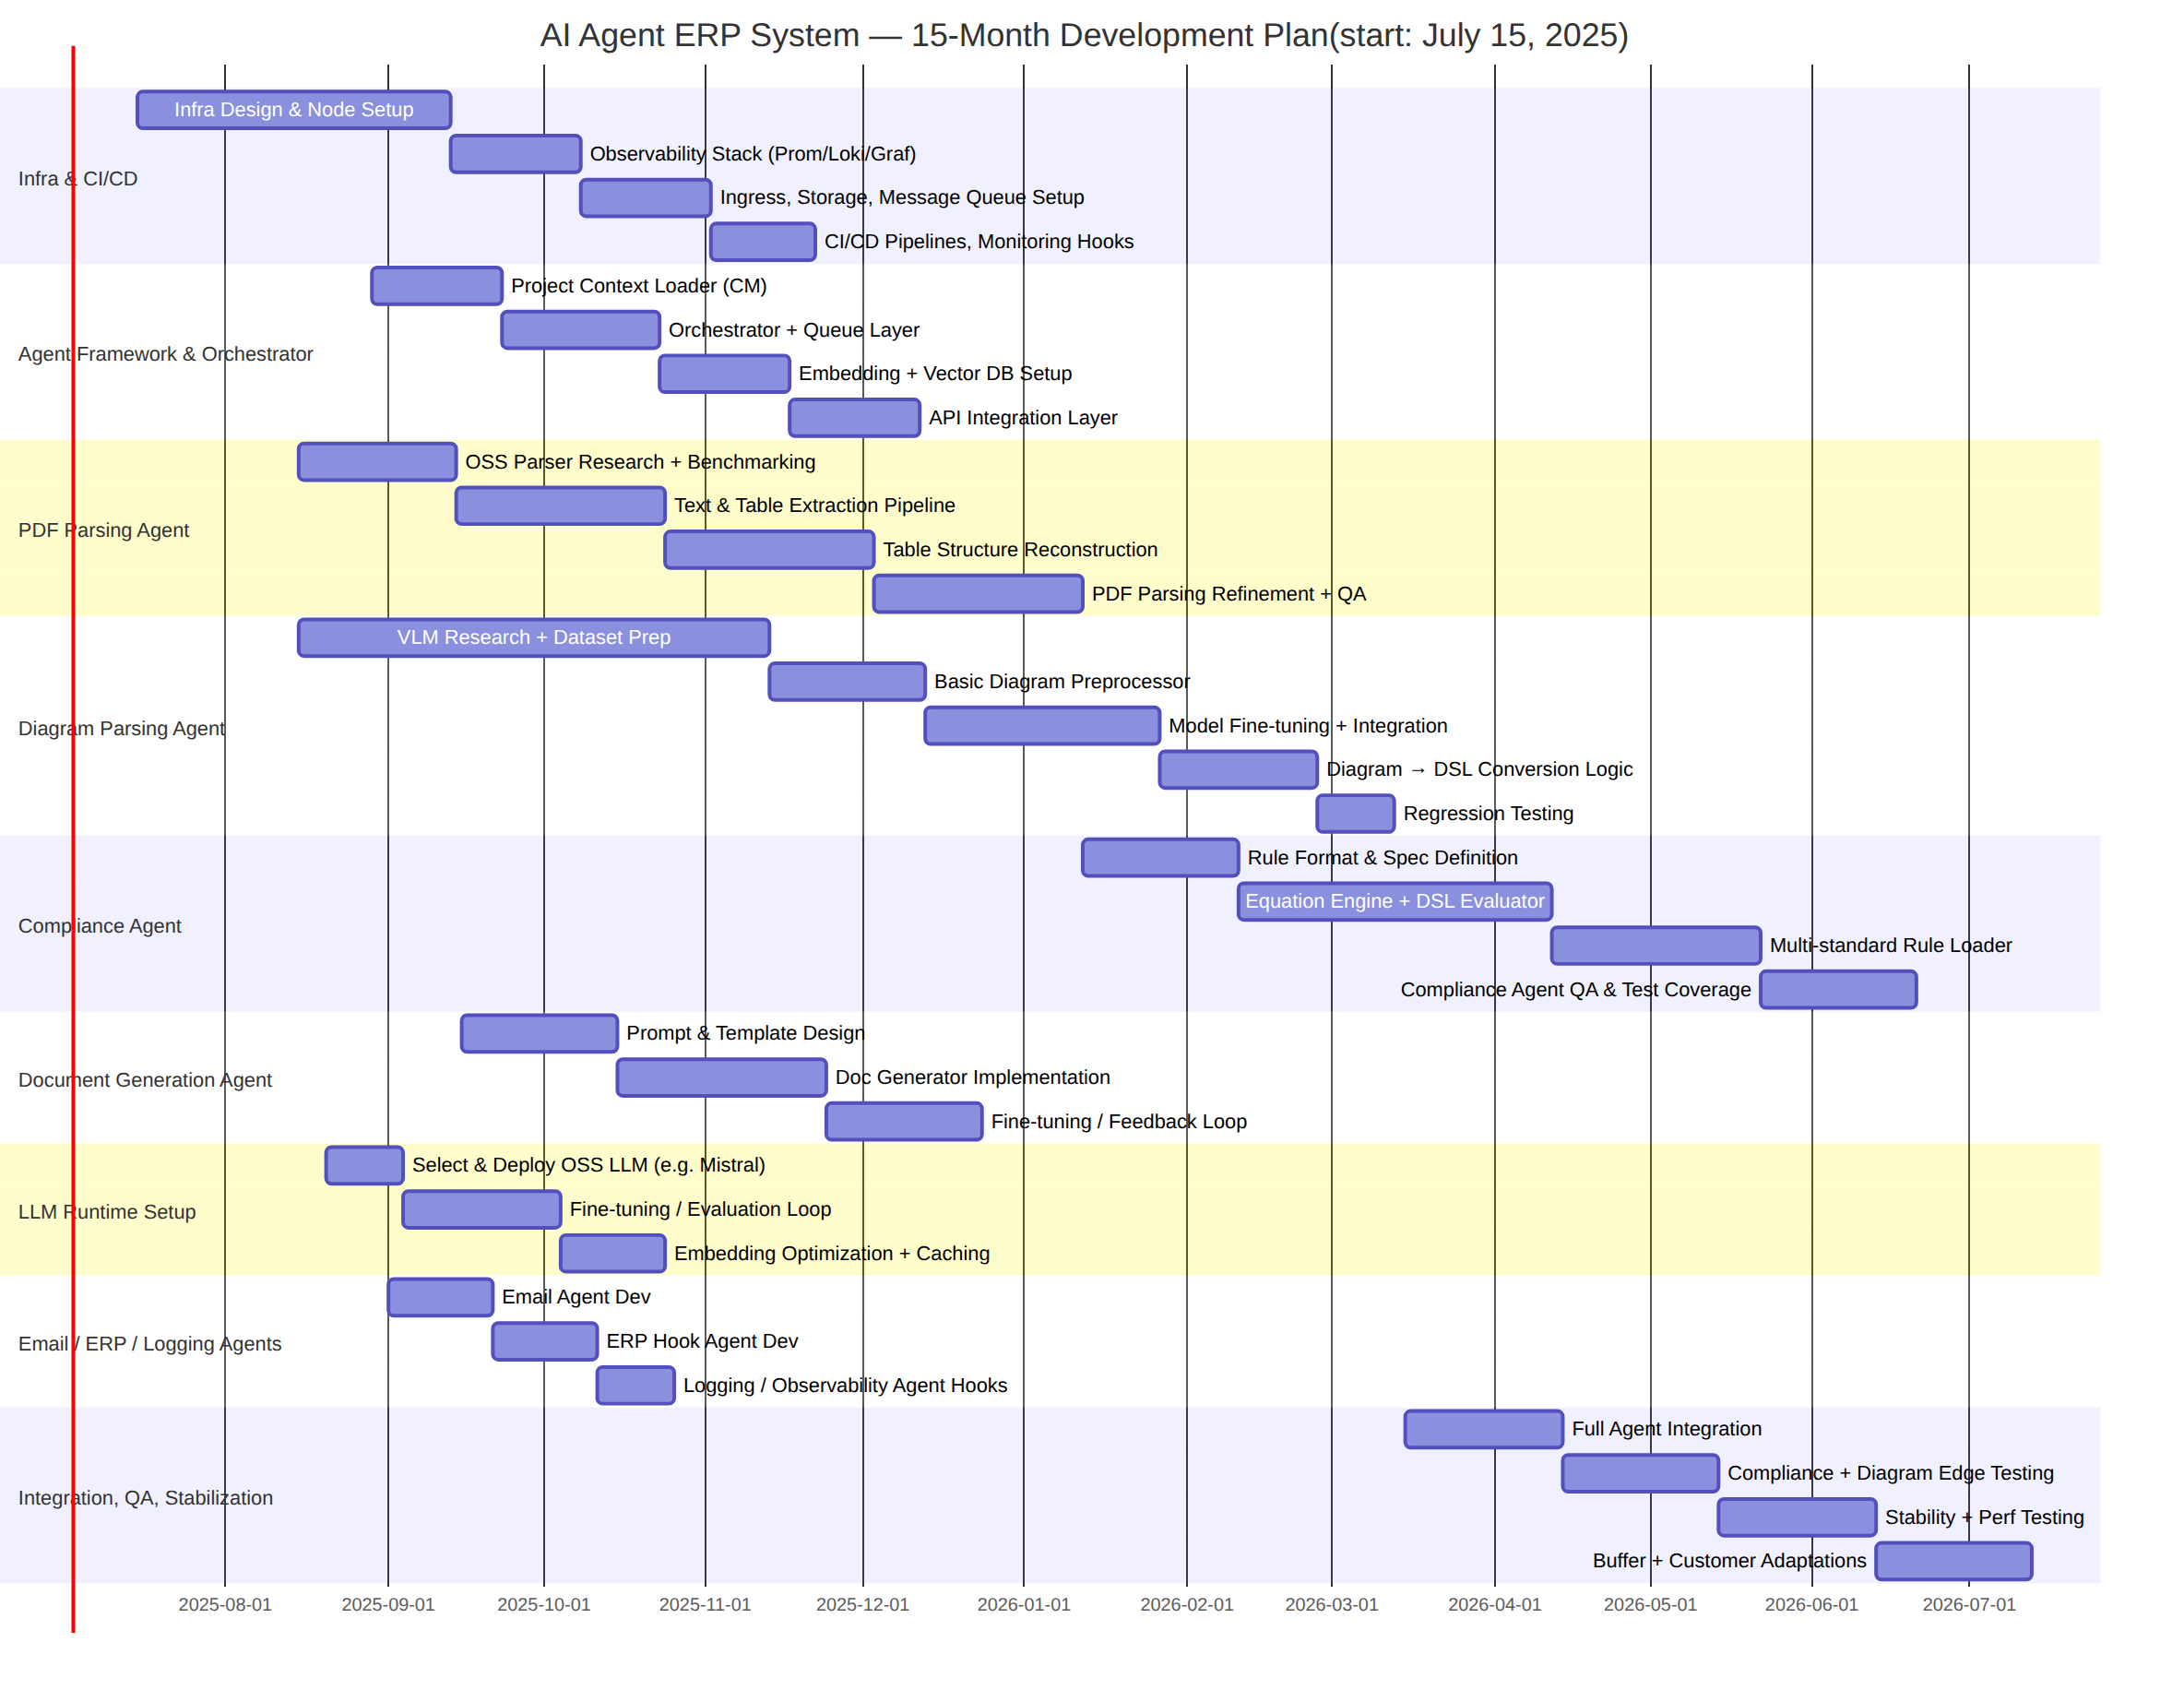
\includegraphics[width=\textwidth,height=0.8\textheight,keepaspectratio]{../../pics/gantt.png}
\caption{AI Agent ERP System 15-Month Development Timeline}
\label{fig:implementation-timeline}
\end{figure}

\section{Development Phases}

\subsection{Phase 1: Infrastructure Foundation (July September 2025)}

\subsubsection{Infrastructure Design \& Node Setup (60 days)}
\begin{itemize}
  \item \textbf{Duration}: July 15 - September 13, 2025
  \item \textbf{Deliverables}:
    \begin{itemize}
      \item Complete hardware procurement and physical server setup
      \item VM distribution strategy implementation with specialized pools
      \item Kubernetes cluster initialization with 3-node control plane
      \item Network configuration with ingress controllers and load balancers
    \end{itemize}
  \item \textbf{Key Milestones}:
    \begin{itemize}
      \item Hardware delivery and data center setup
      \item Hypervisor installation and VM provisioning
      \item Kubernetes control plane deployment
      \item Basic networking and storage configuration
    \end{itemize}
\end{itemize}

\subsubsection{Observability Stack Deployment (25 days)}
\begin{itemize}
  \item \textbf{Duration}: September 14--October 8, 2025
  \item \textbf{Dependencies}: Infrastructure Design completion
  \item \textbf{Deliverables}:
    \begin{itemize}
      \item Prometheus metrics collection and alerting setup
      \item Loki log aggregation deployment
      \item Grafana dashboards and visualization configuration
      \item Jaeger distributed tracing implementation
    \end{itemize}
  \item \textbf{Success Criteria}:
    \begin{itemize}
      \item Full cluster visibility with real-time metrics
      \item Automated alerting for critical system events
      \item Centralized log aggregation across all services
    \end{itemize}
\end{itemize}

\subsubsection{Core Services Setup (25 days)}
\begin{itemize}
  \item \textbf{Duration}: October 9--November 2, 2025
  \item \textbf{Dependencies}: Observability stack completion
  \item \textbf{Deliverables}:
    \begin{itemize}
      \item Ingress controllers and external access configuration
      \item Persistent storage setup with distributed storage layer
      \item Apache Kafka message queue deployment
      \item Redis caching layer implementation
    \end{itemize}
\end{itemize}

\subsubsection{CI/CD Pipeline Implementation (20 days)}
\begin{itemize}
  \item \textbf{Duration}: November 3--November 22, 2025
  \item \textbf{Dependencies}: Core services completion
  \item \textbf{Deliverables}:
    \begin{itemize}
      \item GitOps workflow with ArgoCD deployment
      \item Automated testing pipelines for all components
      \item Container registry and security scanning integration
      \item Deployment monitoring and rollback mechanisms
    \end{itemize}
\end{itemize}

\subsection{Phase 2: Agent Framework Development (August--November 2025)}

\subsubsection{Project Context Loader \& Configuration Management (25 days)}
\begin{itemize}
  \item \textbf{Duration}: August 29--September 22, 2025
  \item \textbf{Parallel Track}: Can start while infrastructure is being finalized
  \item \textbf{Deliverables}:
    \begin{itemize}
      \item Project-scoped knowledge base implementation
      \item Configuration management system for agent parameters
      \item Dynamic context loading mechanisms
      \item Role-based access control for project data
    \end{itemize}
\end{itemize}

\subsubsection{Orchestrator \& Queue Layer (30 days)}
\begin{itemize}
  \item \textbf{Duration}: September 23--October 22, 2025
  \item \textbf{Dependencies}: Context loader completion
  \item \textbf{Deliverables}:
    \begin{itemize}
      \item Central orchestrator service with workflow management
      \item Message queue integration for agent coordination
      \item Request routing and load balancing logic
      \item Dead letter queue handling for failed requests
    \end{itemize}
\end{itemize}

\subsubsection{Embedding \& Vector Database Setup (25 days)}
\begin{itemize}
  \item \textbf{Duration}: October 23--November 16, 2025
  \item \textbf{Dependencies}: Orchestrator completion
  \item \textbf{Deliverables}:
    \begin{itemize}
      \item Qdrant vector database deployment and configuration
      \item Embedding generation pipeline with SentenceTransformers
      \item Semantic search capabilities implementation
      \item Vector index optimization and caching layer
    \end{itemize}
\end{itemize}

\subsubsection{API Integration Layer (25 days)}
\begin{itemize}
  \item \textbf{Duration}: November 17--December 11, 2025
  \item \textbf{Dependencies}: Vector database completion
  \item \textbf{Deliverables}:
    \begin{itemize}
      \item REST/GRPC API gateway implementation
      \item Authentication and authorization middleware
      \item API rate limiting and security controls
      \item External system integration endpoints
    \end{itemize}
\end{itemize}

\subsection{Phase 3: Specialized Agent Development (August 2025--March 2026)}

\subsubsection{PDF Parsing Agent Development}
\begin{itemize}
  \item \textbf{Research Phase} (30 days): August 15--September 13, 2025
    \begin{itemize}
      \item Open-source parser evaluation and benchmarking
      \item Performance testing with representative document samples
      \item Technology stack selection and architecture design
    \end{itemize}
  \item \textbf{Text \& Table Extraction Pipeline} (40 days): September 14--October 23, 2025
    \begin{itemize}
      \item OCR integration with Tesseract and EasyOCR
      \item Table detection and structure recognition
      \item Text extraction with layout preservation
    \end{itemize}
  \item \textbf{Table Structure Reconstruction} (40 days): October 24--December 2, 2025
    \begin{itemize}
      \item Advanced table parsing algorithms
      \item Cell merging and header detection
      \item Data validation and quality assurance
    \end{itemize}
  \item \textbf{Refinement \& Quality Assurance} (40 days): December 3--January 11, 2026
    \begin{itemize}
      \item Accuracy optimization and error handling
      \item Performance tuning and scalability testing
      \item Integration testing with downstream systems
    \end{itemize}
\end{itemize}

\subsubsection{Diagram Parsing Agent Development}
\begin{itemize}
  \item \textbf{VLM Research \& Dataset Preparation} (90 days): August 15--November 13, 2025
    \begin{itemize}
      \item Vision Language Model evaluation and selection
      \item P\&ID and CAD diagram dataset collection and annotation
      \item Training infrastructure setup and optimization
    \end{itemize}
  \item \textbf{Basic Diagram Preprocessor} (30 days): November 14--December 13, 2025
    \begin{itemize}
      \item Image preprocessing and enhancement algorithms
      \item Format normalization and quality optimization
      \item Symbol detection pipeline implementation
    \end{itemize}
  \item \textbf{Model Fine-tuning \& Integration} (45 days): December 14, 2025--January 27, 2026
    \begin{itemize}
      \item Computer vision model training and validation
      \item Spatial analysis integration with Shapely
      \item OCR integration for text and label extraction
    \end{itemize}
  \item \textbf{Diagram to DSL Conversion} (30 days): January 28--February 26, 2026
    \begin{itemize}
      \item NetworkX graph construction algorithms
      \item Equipment list and connectivity analysis
      \item Structured output generation and validation
    \end{itemize}
  \item \textbf{Regression Testing} (15 days): February 27--March 13, 2026
    \begin{itemize}
      \item Comprehensive test suite development
      \item Performance benchmarking and optimization
      \item Edge case validation and error handling
    \end{itemize}
\end{itemize}

\subsubsection{Compliance Agent Development}
\begin{itemize}
  \item \textbf{Rule Format \& Specification Definition} (30 days): January 12--February 10, 2026
    \begin{itemize}
      \item Compliance rule definition language design
      \item Regulatory standard mapping and categorization
      \item Validation framework architecture
    \end{itemize}
  \item \textbf{Equation Engine \& DSL Evaluator} (60 days): February 11--April 11, 2026
    \begin{itemize}
      \item Mathematical equation parsing and evaluation
      \item Domain-specific language interpreter
      \item Rule execution engine with audit logging
    \end{itemize}
  \item \textbf{Multi-standard Rule Loader} (40 days): April 12--May 21, 2026
    \begin{itemize}
      \item Dynamic rule loading from multiple regulatory sources
      \item Version control and rule update mechanisms
      \item Conflict resolution and priority management
    \end{itemize}
  \item \textbf{Quality Assurance \& Test Coverage} (30 days): May 22--June 20, 2026
    \begin{itemize}
      \item Comprehensive test case development
      \item Validation against known compliance scenarios
      \item Performance optimization and error handling
    \end{itemize}
\end{itemize}

\subsubsection{Document Generation Agent Development}
\begin{itemize}
  \item \textbf{Prompt \& Template Design} (30 days): September 15--October 14, 2025
    \begin{itemize}
      \item LLM prompt engineering for document generation
      \item Template system design and implementation
      \item Content guidelines and style consistency
    \end{itemize}
  \item \textbf{Document Generator Implementation} (40 days): October 15--November 23, 2025
    \begin{itemize}
      \item ERP API integration for data fetching
      \item LLM-based content generation pipeline
      \item JSON output formatting and validation
    \end{itemize}
  \item \textbf{Fine-tuning \& Feedback Loop} (30 days): November 24--December 23, 2025
    \begin{itemize}
      \item Content quality optimization and refinement
      \item User feedback integration mechanisms
      \item Performance tuning and scalability testing
    \end{itemize}
\end{itemize}

\subsubsection{LLM Runtime Setup}
\begin{itemize}
  \item \textbf{Model Selection \& Deployment} (15 days): August 20--September 3, 2025
    \begin{itemize}
      \item Open-source LLM evaluation (Mistral, DeepSeek, Llama)
      \item GPU infrastructure optimization for model serving
      \item vLLM deployment and configuration
    \end{itemize}
  \item \textbf{Fine-tuning \& Evaluation} (30 days): September 4--October 3, 2025
    \begin{itemize}
      \item Domain-specific model fine-tuning for ERP context
      \item Performance benchmarking and optimization
      \item Model version management and deployment
    \end{itemize}
  \item \textbf{Embedding Optimization \& Caching} (20 days): October 4--October 23, 2025
    \begin{itemize}
      \item Embedding model optimization for semantic search
      \item Caching layer implementation for performance
      \item Vector database integration and tuning
    \end{itemize}
\end{itemize}

\subsubsection{Supporting Agents Development}
\begin{itemize}
  \item \textbf{Email Agent Development} (20 days): September 1--September 20, 2025
    \begin{itemize}
      \item NLP parsing with DocAI integration
      \item Intent classification and entity extraction
      \item RAG engine integration for context understanding
    \end{itemize}
  \item \textbf{ERP Hook Agent Development} (20 days): September 21--October 10, 2025
    \begin{itemize}
      \item Natural language to ERP API translation
      \item Semantic understanding for equipment queries
      \item Response formatting and user interaction
    \end{itemize}
  \item \textbf{Logging \& Observability Agent Hooks} (15 days): October 11--October 25, 2025
    \begin{itemize}
      \item Comprehensive logging integration
      \item Performance metrics collection
      \item Operational monitoring and alerting
    \end{itemize}
\end{itemize}

\subsection{Phase 4: Integration and Quality Assurance (March 2026--October 2026)}

\subsubsection{Full Agent Integration (30 days)}
\begin{itemize}
  \item \textbf{Duration}: March 15--April 13, 2026
  \item \textbf{Dependencies}: All individual agents completed
  \item \textbf{Deliverables}:
    \begin{itemize}
      \item End-to-end workflow integration testing
      \item Cross-agent communication validation
      \item Performance optimization across the entire system
      \item Integration with external ERP systems
    \end{itemize}
\end{itemize}

\subsubsection{Compliance \& Diagram Edge Testing (30 days)}
\begin{itemize}
  \item \textbf{Duration}: April 14--May 13, 2026
  \item \textbf{Focus Areas}:
    \begin{itemize}
      \item Complex diagram parsing scenarios with edge cases
      \item Multi-standard compliance validation testing
      \item Performance testing with large document sets
      \item Accuracy validation against manual processes
    \end{itemize}
\end{itemize}

\subsubsection{Stability \& Performance Testing (30 days)}
\begin{itemize}
  \item \textbf{Duration}: May 14--June 12, 2026
  \item \textbf{Testing Scope}:
    \begin{itemize}
      \item Load testing with concurrent user scenarios
      \item Memory and resource utilization optimization
      \item Failure recovery and disaster recovery testing
      \item Security penetration testing and vulnerability assessment
    \end{itemize}
\end{itemize}

\subsubsection{Buffer \& Customer Adaptations (30 days)}
\begin{itemize}
  \item \textbf{Duration}: June 13--July 12, 2026
  \item \textbf{Activities}:
    \begin{itemize}
      \item Customer-specific configuration and customization
      \item Documentation finalization and user training materials
      \item Deployment preparation and rollout planning
      \item Final optimizations based on user acceptance testing
    \end{itemize}
\end{itemize}

\section{Risk Mitigation and Contingency Planning}

\subsection{Technical Risks}
\begin{itemize}
  \item \textbf{LLM Performance Issues}: Parallel evaluation of multiple open-source models with fallback options
  \item \textbf{Diagram Parsing Accuracy}: Extended research phase with multiple VLM approaches
  \item \textbf{Integration Complexity}: Modular development approach with well-defined interfaces
  \item \textbf{Hardware Delays}: Early procurement with backup supplier relationships
\end{itemize}

\subsection{Schedule Risks}
\begin{itemize}
  \item \textbf{Parallel Development Streams}: Minimize critical path dependencies
  \item \textbf{Buffer Time Allocation}: 30-day buffer at project end for unforeseen issues
  \item \textbf{Milestone-based Validation}: Regular checkpoint reviews and scope adjustments
  \item \textbf{Resource Flexibility}: Cross-training team members across multiple components
\end{itemize}

\section{Success Metrics and Deliverables}

\subsection{Phase Gate Criteria}
\begin{itemize}
  \item \textbf{Phase 1}: Infrastructure 99.9\% uptime, full observability coverage
  \item \textbf{Phase 2}: API response times < 200ms, successful load balancing
  \item \textbf{Phase 3}: Agent accuracy > 95\%, performance benchmarks met
  \item \textbf{Phase 4}: End-to-end workflows validated, customer acceptance achieved
\end{itemize}

\subsection{Final Deliverables}
\begin{itemize}
  \item \textbf{Production-Ready System}: Fully deployed AI Agent Module with all specialized agents
  \item \textbf{Documentation Suite}: Complete technical documentation, user guides, and operational procedures
  \item \textbf{Training Materials}: Comprehensive training program for administrators and end users
  \item \textbf{Support Framework}: Incident response procedures, maintenance guidelines, and upgrade pathways
\end{itemize}


\chapter{Conclusion}
The AI Agent Module for the Prowiz ERP System represents a comprehensive, modular, and scalable solution for automating process design, compliance, document generation, diagram parsing, email processing, and ERP interaction. This Software Design Document has detailed the architecture, component responsibilities, integration boundaries, infrastructure, deployment strategies, and implementation plan.

With a robust microservices-based architecture, Kubernetes orchestration, and Infrastructure as Code, the system is designed for high availability, security, and operational excellence. The phased implementation plan ensures risk mitigation, quality assurance, and alignment with business objectives.

The next steps involve executing the outlined development phases, rigorous testing, and seamless deployment, followed by continuous monitoring and iterative improvements. Successful implementation will streamline workflows, enhance accuracy, and deliver significant value to all stakeholders within the ERP ecosystem.

\appendix
\chapter{Glossary}
\begin{description}
  \item[AI Agent Module] A modular subsystem providing specialized AI-powered agents for process automation, compliance, document generation, diagram parsing, email processing, and ERP interaction within the Prowiz ERP System.
  \item[API] Application Programming Interface; a set of protocols for building and integrating application software.
  \item[API Gateway] A service that provides a single entry point for API requests, routing them to appropriate backend services.
  \item[ArgoCD] A declarative, GitOps continuous delivery tool for Kubernetes.
  \item[CI/CD] Continuous Integration/Continuous Deployment; automated processes for building, testing, and deploying code.
  \item[Compliance Agent] Specialized agent responsible for validating data against business rules and regulatory standards.
  \item[CPU] Central Processing Unit; the primary component of a computer that performs calculations.
  \item[CUDA] Compute Unified Device Architecture; a parallel computing platform by NVIDIA for GPU acceleration.
  \item[Dead Letter Queue] A message queue for storing messages that cannot be processed successfully.
  \item[DocAI] Document AI; tools or services for automated document analysis using AI.
  \item[Document Generation Agent] Agent that generates narrative and structured documents using LLMs and ERP data.
  \item[DSL] Domain-Specific Language; a computer language specialized to a particular application domain.
  \item[Embedding] A vector representation of data (such as text) used for semantic search and similarity.
  \item[ERP] Enterprise Resource Planning; integrated management of main business processes, often in real-time.
  \item[ERP-Chat Agent] Agent that enables natural language querying and interaction with ERP systems.
  \item[Faiss] Facebook AI Similarity Search; a library for efficient similarity search and clustering of dense vectors.
  \item[GPU] Graphics Processing Unit; specialized hardware for parallel processing, often used in AI workloads.
  \item[Helm] A package manager for Kubernetes applications.
  \item[HMBT] Heat and Material Balance Table; a process engineering document.
  \item[IaC] Infrastructure as Code; managing and provisioning computing infrastructure through machine-readable definition files.
  \item[Jaeger] An open-source distributed tracing system.
  \item[JSON] JavaScript Object Notation; a lightweight data-interchange format.
  \item[Kubernetes] An open-source platform for automating deployment, scaling, and management of containerized applications.
  \item[LangChain] An open-source framework for developing applications powered by language models.
  \item[LangGraph] A workflow orchestration tool for LLMs.
  \item[LangSmith] A tool for tracing and debugging LLM applications.
  \item[Llama] A family of open-source large language models by Meta.
  \item[Loki] A log aggregation system designed for efficiency and scalability.
  \item[LLM] Large Language Model; a machine learning model trained on vast amounts of text data for natural language processing tasks.
  \item[LLM Runtime] The infrastructure and environment for serving and running LLM inference workloads.
  \item[Message Queue] A communication method for exchanging messages between services asynchronously.
  \item[Mistral] An open-source large language model.
  \item[MongoDB] A NoSQL, document-oriented database.
  \item[NLP] Natural Language Processing; a field of AI focused on the interaction between computers and human language.
  \item[OCR] Optical Character Recognition; technology for converting images of text into machine-encoded text.
  \item[PDF] Portable Document Format; a file format for capturing and sending electronic documents.
  \item[PFD] Process Flow Diagram; a type of flowchart that illustrates the relationships between major components in a process.
  \item[P\&ID] Piping and Instrumentation Diagram; a detailed diagram showing the piping and related components of a physical process flow.
  \item[Prometheus] An open-source monitoring and alerting toolkit.
  \item[Qdrant] An open-source vector database for storing and searching embeddings.
  \item[RAG] Retrieval-Augmented Generation; an AI technique combining information retrieval with generative models.
  \item[RBAC] Role-Based Access Control; a method of regulating access to computer or network resources.
  \item[Redis] An in-memory data structure store, used as a database, cache, and message broker.
  \item[REST] Representational State Transfer; an architectural style for designing networked applications.
  \item[SLA] Service Level Agreement; a contract that defines the level of service expected from a service provider.
  \item[SQL] Structured Query Language; a standard language for managing and manipulating databases.
  \item[Terraform] An open-source IaC software tool.
  \item[Tesseract] An open-source OCR engine.
  \item[Vector Database] A database optimized for storing and searching vector embeddings.
  \item[vLLM] An open-source fast and memory-efficient LLM inference engine.
  \item[VM] Virtual Machine; an emulation of a computer system.
  \item[VLM] Vision Language Model; a model that processes both visual and textual data.
  \item[Workflow Orchestrator] A component that manages the execution order and dependencies of tasks or services.
\end{description}

\end{document}
